% =====================================================================
%  Proyecto P2 -- Informe final consolidado
%  Internet de las Cosas (CS5055) -- UTEC 2026-2 -- Grupo 7
% =====================================================================
\documentclass[10pt,twocolumn]{article}

\usepackage[letterpaper,top=1.6cm,bottom=1.7cm,left=1.5cm,right=1.5cm,columnsep=0.6cm]{geometry}
\usepackage[spanish,es-nodecimaldot,es-noshorthands,es-tabla]{babel}
\usepackage[T1]{fontenc}
\usepackage[utf8]{inputenc}
\usepackage{lmodern}
\usepackage{microtype}
\usepackage{amsmath,amssymb}
\usepackage{booktabs,tabularx,array,multirow}
\usepackage{enumitem}
\usepackage{graphicx}
\usepackage{xcolor}
\usepackage{float}
\usepackage{tikz}
\usetikzlibrary{arrows.meta,positioning,fit,shapes.geometric,calc,babel}
\usepackage{titlesec}
\usepackage{fancyhdr}
\usepackage{caption}
\usepackage{balance}
\usepackage{cite}
\usepackage{url}
\usepackage{hyperref}

% --- Paleta verde (misma que la presentación del P1) -------------------
\definecolor{VerdeBase}{HTML}{005A36}
\definecolor{VerdeOscuro}{HTML}{004026}
\definecolor{VerdeMedio}{HTML}{2E7D57}
\definecolor{VerdeSuave}{HTML}{A8D5BD}
\definecolor{VerdeFondo}{HTML}{F2F8F5}
\definecolor{GrisTexto}{HTML}{404040}

\hypersetup{colorlinks=true,linkcolor=VerdeOscuro,citecolor=VerdeOscuro,urlcolor=VerdeMedio}

\setlength{\parindent}{0pt}
\setlength{\parskip}{3.2pt}
\setlist{nosep,leftmargin=*,topsep=2pt}
\renewcommand{\arraystretch}{1.1}
\captionsetup{font=small,labelfont={bf,color=VerdeOscuro}}

\titleformat{\section}{\large\bfseries\color{VerdeOscuro}}{\thesection.}{0.45em}{}[\vspace{-2pt}\color{VerdeMedio}\titlerule]
\titleformat{\subsection}{\normalsize\bfseries\color{GrisTexto}}{\thesubsection}{0.4em}{}
\titleformat{\subsubsection}{\small\bfseries\itshape\color{GrisTexto}}{\thesubsubsection}{0.4em}{}
\titlespacing*{\section}{0pt}{8pt}{4pt}
\titlespacing*{\subsection}{0pt}{6pt}{2pt}
\titlespacing*{\subsubsection}{0pt}{4pt}{1pt}

\pagestyle{fancy}
\fancyhf{}
\fancyhead[L]{\footnotesize Proyecto P2 --- Semana 14 --- Grupo 7}
\fancyhead[R]{\footnotesize Mantenimiento predictivo IoT}
\fancyfoot[C]{\thepage}
\renewcommand{\headrulewidth}{0.3pt}

% --- Utilidades ---------------------------------------------------------
% Texto que el equipo debe completar antes de exportar el PDF final.
\newcommand{\pendiente}[1]{\textcolor{red!70!black}{\textbf{[Completar: #1]}}}
\newcommand{\code}[1]{\texttt{\small #1}}

% Figura que se incluye si el archivo existe; si no, muestra un recuadro
% indicando la ruta esperada (útil para fotos y capturas pendientes).
% #1 ruta con extensión, #2 alto del recuadro, #3 ancho relativo
\newcommand{\imagenopcional}[3]{%
  \IfFileExists{#1}%
    {\includegraphics[width=#3,height=#2,keepaspectratio]{#1}}%
    {\fcolorbox{red!70!black}{red!4}{\parbox[c][#2][c]{\dimexpr#3-2\fboxsep-2\fboxrule}{\centering\small\color{red!70!black}
      \textbf{Imagen pendiente}\\[2pt]\texttt{\detokenize{#1}}}}}}

% --- Estilos TikZ -------------------------------------------------------
\tikzset{
  bloque/.style={draw=VerdeBase, fill=VerdeFondo, rounded corners=2pt, align=center,
                 font=\scriptsize, minimum height=0.9cm, inner sep=3pt},
  nucleo/.style={bloque, fill=VerdeSuave!45, line width=0.9pt},
  nube/.style={bloque, fill=VerdeSuave!25, draw=VerdeOscuro, dashed},
  actuador/.style={bloque, draw=VerdeOscuro, fill=VerdeSuave!80},
  flecha/.style={-{Stealth[length=2mm]}, VerdeOscuro, thick},
  orden/.style={-{Stealth[length=2mm]}, VerdeMedio, thick, dashed},
  etiqueta/.style={font=\tiny, text=black!80, fill=white, inner sep=1pt, align=center},
  % diagrama de flujo
  inicio/.style={draw=VerdeOscuro, fill=VerdeSuave!70, rounded corners=7pt, font=\scriptsize,
                 align=center, minimum width=2.6cm, minimum height=0.6cm},
  proceso/.style={draw=VerdeBase, fill=VerdeFondo, font=\scriptsize, align=center,
                  minimum width=3.4cm, minimum height=0.6cm, text width=3.3cm, inner sep=2pt},
  decision/.style={draw=VerdeOscuro, fill=VerdeSuave!35, diamond, aspect=2.6, font=\scriptsize,
                   align=center, inner sep=0.5pt, text width=2.0cm},
  io/.style={draw=VerdeBase, fill=white, trapezium, trapezium left angle=72, trapezium right angle=108,
             font=\scriptsize, align=center, minimum height=0.6cm, text width=2.8cm, inner sep=2pt},
  linea/.style={-{Stealth[length=1.6mm]}, VerdeOscuro, semithick},
}

% =====================================================================
\begin{document}

\twocolumn[
\begin{center}
{\LARGE\bfseries\color{VerdeOscuro}
Sistema IoT de mantenimiento predictivo para máquinas rotativas
mediante monitoreo multimodal y detección de anomalías\par}

\vspace{6pt}
{\normalsize
Josep Ratzinger Castro Ferrer \quad·\quad Jean Paul Cuzcano Ponce \quad·\quad
Rodrigo Félix Meza Gavilán \quad·\quad Marcelino Maita Vargas\par}

\vspace{3pt}
{\small Docente: Gabriel Andrés Arias Obregón\par}
{\small Internet de las Cosas (CS5055) --- Universidad de Ingeniería y Tecnología (UTEC) --- 2026-2\par}
{\small Sitio web del proyecto: \url{https://claude.ai/artifact/9TY8EvhtF9nVcEp52EMShx\#inicio}\par}
{\small Proyecto P2 --- 13 de noviembre de 2026\par}
\end{center}

\begin{minipage}{\textwidth}
\small
\textbf{Resumen---}
Se presenta el desarrollo e implementación de un prototipo IoT que vigila un ventilador
\textit{brushless} de 12~V como caso de estudio de máquina rotativa. Un ESP32 adquiere
aceleración triaxial (MPU6050), temperatura del motor (DS18B20) y la tensión de salida de un
sensor de corriente de efecto Hall (ACS712), y publica cada lectura mediante MQTT sobre TLS
hacia AWS IoT Core. Una regla de IoT invoca una función AWS Lambda empaquetada como contenedor
que evalúa la lectura con un detector Isolation Forest ajustado con mediciones de referencia
seleccionadas por el estado reportado ENCENDIDO, sin una etiqueta independiente de salud,
registra el resultado en DynamoDB y, tras tres anomalías consecutivas, puede ordenar al ESP32 la
apertura del relé que alimenta al ventilador. El modelo se entrenó con 3\,927 lecturas reales de
operación, con una partición cronológica 70/15/15 y un umbral fijado en el percentil~99 de la
calibración. En el bloque de prueba, que no intervino en el ajuste, el detector marcó como
anómalas el 1.19\,\% de las lecturas; ante perturbaciones sintéticas de validación detectó el
83.1\,\% de las muestras alteradas. Se discuten las limitaciones del muestreo a
1~Hz y la ausencia de fallas etiquetadas, y se proponen mejoras para una siguiente iteración.

\textbf{Palabras clave---}
mantenimiento predictivo, Internet de las cosas, detección de anomalías, Isolation Forest,
ESP32, MQTT, AWS IoT Core, AWS Lambda.
\end{minipage}
\vspace{10pt}
]

% =====================================================================
\section{Introducción}

Ventiladores, bombas, compresores y motores eléctricos sostienen buena parte de los procesos de
ventilación, bombeo y manufactura. Estas máquinas rara vez se detienen sin dar señales previas:
el desbalance, la holgura o el deterioro de los rodamientos modifican la respuesta vibratoria del
equipo, la fricción eleva el consumo eléctrico y el trabajo forzado acumula calor en el
motor~\cite{tiboni2022,lei2018}. Cuando esas señales se observan de forma continua, la
intervención puede planificarse antes de que ocurra la parada.

El Internet de las Cosas (IoT) abarata esta observación continua: un microcontrolador con
conectividad inalámbrica puede leer varios sensores, enviar las mediciones a un servicio en la
nube y recibir de vuelta una orden de actuación~\cite{compare2020}. Sobre esta idea, el presente
proyecto construye un nodo de monitoreo para un ventilador \textit{brushless} de 12~V que combina
tres variables ---vibración, corriente y temperatura---, las analiza con un detector de anomalías
ajustado con mediciones de referencia del equipo reportado como encendido y puede cortar su
alimentación mediante un relé. Ese estado de control no constituye por sí solo una etiqueta
certificada de funcionamiento saludable.

Este informe consolida el perfil presentado en la primera entrega (P1) e incorpora el desarrollo
real del prototipo. Respecto del perfil, se introdujeron dos cambios de diseño que se justifican
en la Sección~\ref{sec:metodologia}: el detector Random Cut Forest (RCF) se sustituyó por
Isolation Forest, y la inferencia, inicialmente prevista en una laptop, se trasladó a una
arquitectura sin servidores en AWS. El trabajo se organizó en cuatro frentes: armado del
hardware, modelo de aprendizaje automático, simulación del circuito en la web y conexión con AWS.

\subsection*{Objetivo general}
Diseñar e implementar un prototipo IoT de bajo costo que detecte anomalías en una máquina rotativa
a partir de la adquisición conjunta de vibración, corriente y temperatura, con comunicación
inalámbrica, inferencia en la nube y parada controlada mediante relé.

\subsection*{Objetivos específicos}
\begin{enumerate}
  \item Integrar el MPU6050, el ACS712 y el DS18B20 con un ESP32 y caracterizar la continuidad y
        estabilidad de sus lecturas.
  \item Construir un conjunto de datos de referencia del ventilador y documentar el criterio
        usado para seleccionarlo.
  \item Entrenar, calibrar y seleccionar un detector de anomalías no supervisado.
  \item Implementar la cadena ESP32--AWS IoT Core--Lambda--DynamoDB y el canal de retorno para la
        orden de parada.
  \item Validar el circuito y el firmware en un simulador web antes del montaje físico.
  \item Encapsular el prototipo separando sensado, control y potencia.
\end{enumerate}

% =====================================================================
\section{Problemática}

Las fallas de origen mecánico en máquinas rotativas ---desbalance, holgura, fricción y
sobrecalentamiento--- evolucionan de forma progresiva, pero en equipos pequeños suelen detectarse
recién cuando la máquina ya se detuvo, con el costo de una parada imprevista y de daños
mayores~\cite{zonta2020,carvalho2019}. La Tabla~\ref{tab:problema} resume por qué las prácticas
habituales no bastan.

\begin{table}[htbp]
\centering
\caption{Prácticas habituales de supervisión y sus limitaciones.}
\label{tab:problema}
\footnotesize
\begin{tabularx}{\columnwidth}{@{}>{\raggedright\arraybackslash}p{2.1cm}>{\raggedright\arraybackslash}X@{}}
\toprule
\textbf{Práctica} & \textbf{Limitación} \\
\midrule
Inspección esporádica & Ofrece solo una fotografía del instante observado; los cambios
respecto del comportamiento normal pasan desapercibidos entre visitas~\cite{carvalho2019,cinar2020}. \\
\addlinespace
Una sola variable & La corriente también varía con la carga, la vibración depende de la
fijación del sensor y la temperatura reacciona tarde; combinarlas reduce la
ambigüedad~\cite{li2017,niu2023}. \\
\addlinespace
Alerta sin respuesta & Si nadie actúa a tiempo, detectar el problema no protege al equipo. \\
\bottomrule
\end{tabularx}
\end{table}

El ventilador elegido no dispone de ningún medio para registrar estas variables, emitir alertas ni
detenerse ante una condición anómala. De ahí surge la pregunta que guía el proyecto:
\textbf{¿puede un sistema IoT de bajo costo reconocer desviaciones del funcionamiento normal de un
ventilador de 12~V a partir de su vibración, corriente y temperatura, y ordenar su parada cuando
la desviación persiste?}

% =====================================================================
\section{Marco teórico}

\subsection{Mantenimiento basado en condición}
El mantenimiento correctivo interviene después de la falla y el preventivo lo hace según un
calendario; el mantenimiento basado en condición, en cambio, decide a partir del estado medido del
activo~\cite{lei2018,zhang2019}. Su cadena típica comprende adquisición, preprocesamiento,
representación del estado y decisión (Fig.~\ref{fig:cbm}). Pronosticar la vida útil remanente
(RUL) exige además historiales de degradación completos~\cite{lei2018}, por lo que este proyecto
se limita a detectar desviaciones respecto de una línea base.

\begin{figure}[H]
\centering
\begin{tikzpicture}[node distance=0.3cm]
  \node[bloque, text width=1.3cm] (a) {Adquisición};
  \node[bloque, text width=1.45cm, right=of a] (b) {Preproce\-samiento};
  \node[bloque, text width=1.4cm, right=of b] (c) {Represen\-tación del estado};
  \node[nucleo, text width=1.1cm, right=of c] (d) {Decisión};
  \draw[flecha] (a) -- (b); \draw[flecha] (b) -- (c); \draw[flecha] (c) -- (d);
\end{tikzpicture}
\caption{Cadena del mantenimiento basado en condición, adaptada de~\cite{lei2018,zhang2019}.}
\label{fig:cbm}
\end{figure}

\subsection{Variables monitoreadas}

\textbf{Vibración.} El MPU6050 es un acelerómetro MEMS triaxial con convertidor de 16~bits y
rangos de $\pm2$ a $\pm16\,g$~\cite{mpu6050}. Con el sensor en reposo, cada eje registra la
proyección de la gravedad; durante la operación, las fluctuaciones alrededor de ese valor reflejan
la vibración transmitida a la carcasa. La magnitud
$a_m=\sqrt{a_x^2+a_y^2+a_z^2}$ y los indicadores estadísticos por ventana, como el valor RMS y el
factor de cresta, son descriptores habituales del dominio del tiempo~\cite{tiboni2022}.

\textbf{Corriente.} El ACS712 entrega una tensión proporcional a la corriente que atraviesa su
conductor interno:
\begin{equation}
  V_{\mathrm{out}} = V_0 + S\,I ,
  \label{eq:acs}
\end{equation}
donde $V_0\approx V_{CC}/2$ es la salida en reposo y $S=185$~mV/A para la versión de
5~A~\cite{acs712}. La firma de corriente es una técnica no invasiva que revela alteraciones
eléctricas y mecánicas, aunque depende del régimen de operación~\cite{niu2023,benbouzid2000}.

\textbf{Temperatura.} El DS18B20 es un termómetro digital 1-Wire con exactitud de
$\pm0.5\,^{\circ}$C entre $-10$ y $85\,^{\circ}$C~\cite{ds18b20}. Su dinámica es lenta, de modo
que confirma la acumulación de calor más que anticiparla.

\subsection{Detección de anomalías con Isolation Forest}
Isolation Forest parte de una observación simple: los datos anómalos son escasos y distintos, por
lo que se aíslan con menos particiones aleatorias que los normales~\cite{liu2008,liu2012}. El
algoritmo construye un conjunto de árboles; en cada nodo elige al azar una variable y un punto de
corte. Si $h(x)$ es la profundidad a la que queda aislada la observación $x$, el puntaje de
anomalía es
\begin{equation}
  s(x,\psi) = 2^{-\frac{E[h(x)]}{c(\psi)}}, \qquad
  c(\psi) = 2H(\psi-1) - \frac{2(\psi-1)}{\psi},
  \label{eq:iforest}
\end{equation}
donde $\psi$ es el tamaño de submuestra de cada árbol, $H(i)\approx\ln(i)+0.5772$ y $c(\psi)$ es
la profundidad media de una búsqueda fallida en un árbol binario~\cite{liu2008}. Un valor de $s$
cercano a 1 indica una observación fácil de aislar; valores claramente menores que 0.5 corresponden
a datos típicos. El método solo necesita datos de operación normal, lo que lo hace adecuado cuando
no existe un catálogo de fallas etiquetadas.

Random Cut Forest, propuesto en el P1, pertenece a la misma familia de particiones aleatorias,
pero mide cuánto cambia la estructura del árbol al insertar un punto y está diseñado para
actualizarse en flujo~\cite{guha2016}. Ambos métodos no son equivalentes; la elección final se
discute en la Sección~\ref{sec:metodologia}.

\subsection{Comunicación IoT y procesamiento en la nube}
MQTT es un protocolo de publicación/suscripción ligero: los dispositivos publican mensajes en
\emph{tópicos} y un \emph{broker} los entrega a los suscriptores~\cite{mqtt311,mishra2020}. AWS IoT
Core actúa como broker gestionado y exige autenticación mutua TLS con certificados X.509 en el
puerto 8883~\cite{awsiot}. Sus reglas, escritas en una variante de SQL, filtran los mensajes de un
tópico y los encaminan a otros servicios, como AWS Lambda~\cite{awsrules}. Lambda ejecuta código
bajo demanda sin administrar servidores y admite imágenes de contenedor de hasta
10~GB~\cite{awslambda}, lo que permite desplegar bibliotecas de aprendizaje automático cuyo
tamaño excede el de un paquete comprimido convencional.

% =====================================================================
\section{Estado del arte}
\label{sec:arte}

Se revisaron doce trabajos publicados entre 2019 y 2023, agrupados en cuatro líneas: monitoreo de
condición de máquinas rotativas, aprendizaje automático para mantenimiento predictivo, detección
de anomalías no supervisada e infraestructura IoT. La Tabla~\ref{tab:arte} sintetiza su aporte al
prototipo.

\subsection{Monitoreo de máquinas rotativas}

Tiboni \emph{et al.}~\cite{tiboni2022} revisan el monitoreo de condición basado en vibraciones y
lo descomponen en medición, procesamiento de señal, extracción de características y diagnóstico.
Concluyen que el desempeño del diagnóstico depende tanto de la calidad de la adquisición
---ubicación y fijación del sensor, frecuencia de muestreo--- como del algoritmo. Este resultado
motivó a fijar rígidamente el MPU6050 a la carcasa y a verificar la estabilidad de sus lecturas
antes de entrenar el modelo; también explica la principal limitación encontrada (Sección~\ref{sec:discusion}).

Niu \emph{et al.}~\cite{niu2023} revisan el diagnóstico de motores mediante firmas de corriente.
Destacan que la corriente se mide sin intervenir mecánicamente el equipo y que aporta información
complementaria a la vibración, aunque también varía con la carga y la velocidad. Por ello, en el
prototipo la corriente se interpreta junto a las otras variables y no como indicador aislado de
falla.

Lei \emph{et al.}~\cite{lei2020} revisan tres décadas de aprendizaje automático aplicado al
diagnóstico de fallas en maquinaria, desde los clasificadores con características manuales hasta
el aprendizaje profundo y la transferencia entre máquinas. Señalan que la mayoría de los estudios
depende de bancos de prueba con fallas etiquetadas, situación poco realista en la industria. Esta
observación respalda el uso de un enfoque no supervisado cuando, como aquí, solo se dispone de
operación normal.

\subsection{Aprendizaje automático para mantenimiento predictivo}

Carvalho \emph{et al.}~\cite{carvalho2019} realizan una revisión sistemática de métodos de
aprendizaje automático aplicados al mantenimiento predictivo y encuentran que Random Forest, las
redes neuronales y las máquinas de soporte vectorial son los más usados, casi siempre en modo
supervisado. Subrayan que la elección del método debe responder a los datos disponibles; en este
proyecto, la falta de fallas etiquetadas descarta los clasificadores supervisados.

Zhang \emph{et al.}~\cite{zhang2019} clasifican los métodos dirigidos por datos para mantenimiento
predictivo en modelos estadísticos, de aprendizaje automático y de aprendizaje profundo, y
describen una arquitectura común de adquisición, preprocesamiento, modelado y decisión. Esta
estructura en capas es la base de la figura metodológica del prototipo (Fig.~\ref{fig:arte}).

Zonta \emph{et al.}~\cite{zonta2020} revisan el mantenimiento predictivo en el contexto de la
Industria 4.0 y proponen una taxonomía que distingue el nivel de monitoreo, el tipo de modelo y la
forma de actuación. Identifican la integración del modelo con el proceso de decisión como uno de
los retos abiertos. El prototipo responde a ese reto cerrando el lazo: la inferencia en la nube
puede devolver una orden al dispositivo.

Çınar \emph{et al.}~\cite{cinar2020} analizan aplicaciones de aprendizaje automático para
mantenimiento predictivo orientadas a la manufactura sostenible y concluyen que el valor del
modelo depende de su integración con la cadena de datos y con una necesidad operativa concreta.
Este criterio orientó la priorización: primero un flujo de datos estable y luego la sofisticación
del algoritmo.

Serradilla \emph{et al.}~\cite{serradilla2022} comparan modelos de aprendizaje profundo para
mantenimiento predictivo y destacan su exigencia de datos y de cómputo, así como la dificultad de
interpretar sus salidas. Con apenas una hora de datos de operación y un despliegue en Lambda, un
modelo profundo no resultaba justificable; un ensamble de árboles ligero se ajustaba mejor al
volumen de datos y a la infraestructura.

\subsection{Detección de anomalías no supervisada}

Pang \emph{et al.}~\cite{pang2021} revisan la detección de anomalías con aprendizaje profundo y
caracterizan el problema por la escasez de anomalías etiquetadas, su heterogeneidad y el
desbalance de clases. Recomiendan establecer líneas base con métodos clásicos antes de emplear
redes profundas; en el proyecto, Isolation Forest cumple ese papel.

Hariri \emph{et al.}~\cite{hariri2021} analizan Isolation Forest y muestran que sus cortes
paralelos a los ejes generan artefactos en el mapa de puntajes, que corrigen con cortes de
pendiente aleatoria (\emph{Extended Isolation Forest}). Este hallazgo justifica escalar las
variables antes del detector y advierte que las fronteras de decisión en proyecciones como PCA
deben interpretarse con cautela.

\subsection{Infraestructura IoT}

Compare \emph{et al.}~\cite{compare2020} discuten los desafíos del mantenimiento predictivo
habilitado por IoT: calidad y continuidad de los datos, gestión de grandes volúmenes, ciberseguridad
y la necesidad de mantener decisiones locales ante fallas de comunicación. De este trabajo se
adoptaron dos decisiones: autenticación con certificados en cada dispositivo y la conservación del
control local del relé en el ESP32.

Mishra y Kertesz~\cite{mishra2020} revisan el uso de MQTT en sistemas IoT y máquina a máquina, y
lo comparan con alternativas como CoAP y AMQP. Destacan su bajo consumo de ancho de banda, los
niveles de calidad de servicio y su adopción por las principales plataformas en la nube. Esto
sustentó la elección de MQTT sobre TLS como protocolo entre el ESP32 y AWS IoT Core.

\begin{table*}[t]
\centering
\caption{Síntesis del estado del arte y decisiones de diseño derivadas.}
\label{tab:arte}
\footnotesize
\renewcommand{\arraystretch}{1.15}
\begin{tabularx}{\textwidth}{@{}>{\raggedright\arraybackslash}p{2.7cm}>{\raggedright\arraybackslash}p{2.6cm}>{\raggedright\arraybackslash}X>{\raggedright\arraybackslash}X@{}}
\toprule
\textbf{Trabajo} & \textbf{Línea} & \textbf{Hallazgo relevante} & \textbf{Decisión en el prototipo} \\
\midrule
Tiboni \emph{et al.}, 2022~\cite{tiboni2022} & Vibración en máquinas rotativas &
El diagnóstico depende de la adquisición, no solo del algoritmo. &
Fijación rígida del MPU6050; verificar estabilidad antes de entrenar. \\
Niu \emph{et al.}, 2023~\cite{niu2023} & Firma de corriente &
Medición no invasiva y complementaria, sensible al régimen. &
Corriente como variable conjunta, no como criterio aislado. \\
Lei \emph{et al.}, 2020~\cite{lei2020} & ML para diagnóstico &
La mayoría de estudios requiere fallas etiquetadas. &
Enfoque no supervisado entrenado con operación normal. \\
Carvalho \emph{et al.}, 2019~\cite{carvalho2019} & ML para PdM &
Predominan métodos supervisados; el método depende de los datos. &
Descartar clasificadores supervisados. \\
Zhang \emph{et al.}, 2019~\cite{zhang2019} & Métodos dirigidos por datos &
Arquitectura en capas: adquisición, preprocesamiento, modelo, decisión. &
Estructura del sistema (Fig.~\ref{fig:arte}). \\
Zonta \emph{et al.}, 2020~\cite{zonta2020} & PdM en Industria 4.0 &
Integrar el modelo con la decisión es un reto abierto. &
Lazo cerrado: la nube puede ordenar la parada. \\
Çınar \emph{et al.}, 2020~\cite{cinar2020} & ML y manufactura sostenible &
El valor del modelo depende de la cadena de datos. &
Priorizar flujo de datos estable sobre complejidad. \\
Serradilla \emph{et al.}, 2022~\cite{serradilla2022} & Aprendizaje profundo para PdM &
Alta exigencia de datos y cómputo, baja interpretabilidad. &
Modelo ligero de árboles desplegable en Lambda. \\
Pang \emph{et al.}, 2021~\cite{pang2021} & Detección de anomalías &
Escasez de anomalías etiquetadas; usar líneas base clásicas. &
Isolation Forest como detector de referencia. \\
Hariri \emph{et al.}, 2021~\cite{hariri2021} & Isolation Forest &
Cortes paralelos a ejes generan artefactos de puntaje. &
Escalado robusto previo; PCA solo para visualizar. \\
Compare \emph{et al.}, 2020~\cite{compare2020} & IoT para PdM &
Continuidad de datos, seguridad y decisión local. &
Certificados X.509; relé controlable localmente. \\
Mishra y Kertesz, 2020~\cite{mishra2020} & Protocolo MQTT &
Ligero, con QoS y soporte en plataformas en la nube. &
MQTT sobre TLS hacia AWS IoT Core. \\
\bottomrule
\end{tabularx}
\end{table*}

En conjunto, la literatura respalda tres elementos del prototipo: la combinación de señales
complementarias, el uso de detección no supervisada cuando no hay fallas etiquetadas y la
integración del modelo con un mecanismo de actuación. La brecha que aborda el proyecto no es
algorítmica, sino de integración: demostrar esta cadena completa con componentes de bajo costo y
servicios gestionados en la nube, y documentar con honestidad hasta dónde llega su validación.

% =====================================================================
\section{Metodología y desarrollo del proyecto}
\label{sec:metodologia}

\subsection{Planteamiento del sistema}

Siguiendo la arquitectura en capas descrita en~\cite{zhang2019,compare2020}, el sistema se
organizó en cuatro niveles: percepción, borde, nube y actuación. La Fig.~\ref{fig:arte} muestra
cómo cada capa de la literatura se materializa en un componente concreto del prototipo.

\begin{figure*}[t]
\centering
\begin{tikzpicture}[node distance=0.35cm and 0.55cm]
  % fila superior: capas según la literatura
  \node[bloque, text width=2.7cm, fill=white] (l1) {\textbf{Adquisición}\\señales físicas del activo};
  \node[bloque, text width=2.7cm, fill=white, right=of l1] (l2) {\textbf{Preprocesamiento}\\en el borde y transmisión};
  \node[bloque, text width=2.7cm, fill=white, right=of l2] (l3) {\textbf{Modelado}\\puntaje de anomalía};
  \node[bloque, text width=2.7cm, fill=white, right=of l3] (l4) {\textbf{Decisión}\\persistencia y criterio};
  \node[bloque, text width=2.7cm, fill=white, right=of l4] (l5) {\textbf{Actuación}\\protección del equipo};
  \foreach \a/\b in {l1/l2,l2/l3,l3/l4,l4/l5} \draw[flecha] (\a) -- (\b);
  % fila inferior: implementación
  \node[nucleo, text width=2.7cm, below=0.9cm of l1] (p1) {MPU6050 · ACS712 · DS18B20\\sobre el ventilador};
  \node[nucleo, text width=2.7cm, below=0.9cm of l2] (p2) {ESP32: lectura completa,\\JSON y MQTT/TLS};
  \node[nucleo, text width=2.7cm, below=0.9cm of l3] (p3) {Lambda: escalado robusto\\+ Isolation Forest};
  \node[nucleo, text width=2.7cm, below=0.9cm of l4] (p4) {DynamoDB: contador\\de 3 anomalías seguidas};
  \node[nucleo, text width=2.7cm, below=0.9cm of l5] (p5) {Orden OFF $\rightarrow$ relé\\corta 12 V};
  \foreach \a/\b in {p1/p2,p2/p3,p3/p4,p4/p5} \draw[flecha] (\a) -- (\b);
  \foreach \i in {1,...,5} \draw[dotted, VerdeMedio, thick] (l\i) -- (p\i);
  \node[font=\scriptsize\itshape, anchor=east] at ($(l1.west)+(-0.15,0)$) {Literatura};
  \node[font=\scriptsize\itshape, anchor=east] at ($(p1.west)+(-0.15,0)$) {Prototipo};
\end{tikzpicture}
\caption{Figura explicativa basada en el estado del arte: las capas genéricas del mantenimiento
predictivo dirigido por datos~\cite{zhang2019,compare2020} (arriba) y su implementación en el
prototipo (abajo).}
\label{fig:arte}
\end{figure*}

El diagrama de bloques completo del sistema se presenta en la Fig.~\ref{fig:bloques}. El ESP32 lee
los tres sensores y publica cada lectura completa en el tópico \code{esp32/pub} de AWS IoT Core.
Una regla de IoT reenvía el mensaje a una función Lambda, que calcula el puntaje de anomalía,
almacena la predicción y el último estado del dispositivo en DynamoDB. Una segunda función
Lambda, expuesta como API HTTP, entrega esos datos al monitor web y al gemelo digital.
Si se acumulan tres anomalías consecutivas con el ventilador encendido, la función prepara la orden
\code{\{"message":"OFF"\}} y la publica en \code{esp32/sub}, tópico al que el ESP32 está suscrito
para abrir el relé. En paralelo, la laptop se usa fuera de línea para registrar el conjunto de datos
de entrenamiento y generar el modelo.

\begin{figure*}[t]
\centering
\resizebox{\textwidth}{!}{%
\begin{tikzpicture}[node distance=0.5cm and 0.8cm]
  \node[bloque, minimum width=2.2cm, minimum height=1.3cm] (fan) {\textbf{Ventilador}\\Delta AFB0812SH\\12 V · 0.6 A};
  \node[bloque, minimum width=2.1cm, right=1.3cm of fan] (acs) {\textbf{ACS712}\\corriente};
  \node[bloque, minimum width=2.1cm, above=of acs] (mpu) {\textbf{MPU6050}\\vibración};
  \node[bloque, minimum width=2.1cm, below=of acs] (ds) {\textbf{DS18B20}\\temperatura};
  \node[nucleo, minimum width=2.8cm, minimum height=2.0cm, right=1.3cm of acs] (esp) {\textbf{ESP32}\\lectura de sensores\\JSON + MQTT/TLS\\control del relé};
  \node[actuador, minimum width=2.1cm, below=1.2cm of esp] (rele) {\textbf{Relé 1 canal}\\activo en bajo};
  % nube
  \node[bloque, minimum width=2.6cm, minimum height=1.3cm, right=2.2cm of esp] (iot) {\textbf{AWS IoT Core}\\broker MQTT\\regla SQL};
  \node[bloque, minimum width=2.6cm, minimum height=1.3cm, right=1.3cm of iot] (lam) {\textbf{AWS Lambda}\\contenedor\\Isolation Forest};
  \node[bloque, minimum width=2.4cm, above=0.7cm of lam] (ddb) {\textbf{DynamoDB}\\predicciones\\y contador};
  \node[bloque, minimum width=2.4cm, right=0.9cm of lam] (ui) {\textbf{Visualización}\\API HTTP (Lambda)\\monitor web y gemelo};
  \node[font=\scriptsize\bfseries, text=VerdeOscuro, anchor=north west] (cl) at ($(iot.north west)+(0,1.75)$) {Nube AWS};
  \node[draw=VerdeOscuro, dashed, rounded corners, inner sep=6pt, fit=(iot)(lam)(ddb)(ui)(cl)] {};
  % entrenamiento fuera de línea
  \node[bloque, minimum width=2.6cm, fill=white, below=2.0cm of lam] (lap) {\textbf{Laptop} (fuera de línea)\\registro serie $\rightarrow$ CSV\\entrenamiento $\rightarrow$ \code{.joblib}};

  \draw[flecha] (fan.north) |- node[pos=0.75, above, etiqueta]{montaje rígido} (mpu.west);
  \draw[flecha] (fan.east) -- node[above, etiqueta]{en serie 12 V} (acs.west);
  \draw[flecha] (fan.south) |- node[pos=0.75, below, etiqueta]{contacto con motor} (ds.west);
  \draw[flecha] (mpu.east) -- node[above, sloped, etiqueta]{I$^2$C} (esp.north west);
  \draw[flecha] (acs.east) -- node[above, etiqueta]{ADC1} (esp.west);
  \draw[flecha] (ds.east) -- node[below, sloped, etiqueta]{1-Wire} (esp.south west);
  \draw[flecha] ([yshift=5pt]esp.east) -- node[above, etiqueta]{Wi-Fi · MQTT/TLS\\\code{esp32/pub}} ([yshift=5pt]iot.west);
  \draw[orden] ([yshift=-10pt]iot.west) -- node[below, etiqueta]{\code{esp32/sub}\\orden OFF} ([yshift=-10pt]esp.east);
  \draw[flecha] ([yshift=8pt]iot.east) -- node[above, etiqueta]{regla} ([yshift=8pt]lam.west);
  \draw[orden] ([yshift=-8pt]lam.west) -- node[below, etiqueta]{OFF} ([yshift=-8pt]iot.east);
  \draw[flecha] (lam) -- (ddb);
  \draw[flecha] (ddb) -| node[pos=0.25, above, etiqueta]{lectura} (ui);
  \draw[flecha, dotted] (esp.south east) |- node[pos=0.75, below, etiqueta]{USB serie (conjunto de datos)} (lap.west);
  \draw[flecha, dotted] (lap.north) -- node[right, etiqueta]{modelo en la imagen} (lam.south);
  \draw[flecha] (esp.south) -- node[right, etiqueta]{GPIO26} (rele.north);
  \draw[orden] (rele.west) -| node[pos=0.25, below, etiqueta]{corta la alimentación de 12 V} ([xshift=-0.5cm]fan.south);
\end{tikzpicture}}
\caption{Diagrama de bloques del sistema implementado. Las flechas continuas representan datos;
las discontinuas, la cadena de actuación; las punteadas, el flujo de entrenamiento fuera de
línea.}
\label{fig:bloques}
\end{figure*}

\subsection{Componentes y especificaciones}

La Tabla~\ref{tab:componentes} lista los componentes del prototipo y la Tabla~\ref{tab:requisitos}
muestra cómo se cubren los requisitos mínimos del curso.

\begin{table}[htbp]
\centering
\caption{Componentes principales del prototipo.}
\label{tab:componentes}
\scriptsize
\begin{tabularx}{\columnwidth}{@{}>{\raggedright\arraybackslash}p{1.6cm}>{\raggedright\arraybackslash}X@{}}
\toprule
\textbf{Elemento} & \textbf{Función y especificaciones} \\
\midrule
ESP32 DevKit V1 & Microcontrolador de doble núcleo hasta 240~MHz, Wi-Fi 2.4~GHz, I$^2$C y ADC
SAR de 12~bits~\cite{esp32}. Adquisición, comunicación y control del relé. \\
\addlinespace
MPU6050 & Acelerómetro y giróscopo MEMS triaxial, ADC de 16~bits, $\pm2$ a $\pm16\,g$,
interfaz I$^2$C~\cite{mpu6050}. Fijado a la carcasa. \\
\addlinespace
ACS712 (5~A) & Sensor de corriente de efecto Hall, aislado, 185~mV/A, alimentado a
5~V~\cite{acs712}. En serie con la línea de 12~V. \\
\addlinespace
DS18B20 & Termómetro digital 1-Wire, 9--12~bits, $\pm0.5\,^{\circ}$C~\cite{ds18b20}. En contacto
con el cuerpo del motor. \\
\addlinespace
Relé de 1 canal & Módulo con etapa de manejo, activo en nivel bajo. Interrumpe los 12~V del
ventilador. \\
\addlinespace
Ventilador & Delta AFB0812SH, \textit{brushless}, 12~V, 0.6~A, 4 hilos, 80$\times$80$\times$25~mm.
Máquina rotativa bajo prueba. \\
\addlinespace
Alimentación & Fuente de 12~V DC para el ventilador; USB para el ESP32. \\
\addlinespace
Enclosure & Caja no conductora que aloja ESP32, relé y ACS712, separando señal y potencia. \\
\bottomrule
\end{tabularx}
\end{table}

\begin{table}[htbp]
\centering
\caption{Cumplimiento de los requisitos mínimos.}
\label{tab:requisitos}
\scriptsize
\begin{tabularx}{\columnwidth}{@{}>{\raggedright\arraybackslash}p{2.0cm}>{\raggedright\arraybackslash}X@{}}
\toprule
\textbf{Requisito} & \textbf{Implementación} \\
\midrule
3 sensores & MPU6050, ACS712 y DS18B20. \\
1 actuador & Relé de 1 canal sobre la alimentación del ventilador. \\
Comunicación inalámbrica & Wi-Fi 2.4~GHz del ESP32 con MQTT sobre TLS hacia AWS IoT Core. \\
Interfaz con procesamiento previo & Resultados publicados por la Lambda (puntaje, umbral,
percentil, contador), guardados en DynamoDB y consultables mediante una API HTTP desde un
monitor web; el ESP32 promedia 64
muestras del ACS712 y filtra lecturas incompletas antes de publicar. \\
Enclosure & Caja que separa la electrónica de control de la línea de potencia. \\
\bottomrule
\end{tabularx}
\end{table}

\subsection{Cambios respecto del perfil (P1)}

\textbf{De RCF a Isolation Forest.} El P1 proponía Random Cut Forest. Su implementación de
referencia en AWS forma parte de SageMaker~\cite{awsrcf}, lo que implica mantener un punto de
inferencia dedicado con costo por hora. Isolation Forest pertenece a la misma familia de
particiones aleatorias~\cite{liu2008}, está disponible en scikit-learn~\cite{sklearn}, se entrena
en segundos sobre CPU y su artefacto entrenado cabe dentro de una imagen de Lambda, que solo
consume recursos cuando llega un mensaje.

\textbf{De la laptop a AWS.} El P1 dejaba la nube como ampliación opcional. Durante el desarrollo
se priorizó porque elimina la dependencia de una laptop encendida en la misma red, aporta
autenticación por certificado y deja un registro persistente de cada predicción. La laptop se
mantuvo para la captura del conjunto de datos y el entrenamiento.

\subsection{Organización del trabajo}

El desarrollo se dividió en cuatro frentes que convergen en el sistema de la
Fig.~\ref{fig:bloques} y que estructuran la Sección~\ref{sec:implementacion}:
\begin{enumerate}
  \item \textbf{Armado:} conexiones, firmware del ESP32, montaje de sensores y enclosure.
  \item \textbf{Modelo de aprendizaje automático:} preparación del conjunto de datos,
        entrenamiento, selección y evaluación del detector.
  \item \textbf{Simulación web:} validación del circuito y del firmware antes del montaje físico.
  \item \textbf{Conexión AWS:} registro del dispositivo, regla de IoT, Lambda, DynamoDB y canal
        de retorno de la orden de parada.
\end{enumerate}

\subsection{Procedimiento experimental}
\begin{enumerate}
  \item Verificar en el simulador web el conexionado y la lógica del firmware.
  \item Montar los sensores sobre el ventilador y comprobar cada lectura por puerto serie.
  \item Registrar una sesión prolongada de operación normal para formar el conjunto de datos.
  \item Entrenar el detector con una partición cronológica y calibrar el umbral con datos no
        vistos.
  \item Evaluar la tasa de alertas en un bloque de prueba reservado y la sensibilidad ante
        perturbaciones controladas.
  \item Verificar de extremo a extremo la publicación MQTT, la inferencia en Lambda y la
        respuesta del relé ante la orden \code{OFF}.
\end{enumerate}

% =====================================================================
\section{Implementación}
\label{sec:implementacion}

\subsection{Armado del prototipo}

El armado comenzó en la protoboard, donde se conectó el ESP32 con los sensores. Después se incorporó el circuito de alimentación del ventilador y se preparó un programa de prueba para comprobar el conjunto desde el monitor serie.

\subsubsection{Interconexión de componentes}
Primero se conectó el ESP32 por USB a la computadora y se distribuyeron los 3.3~V y GND en la protoboard. A esa alimentación se conectaron la sonda DS18B20 y el MPU6050. La sonda se enlazó al GPIO4 mediante 1-Wire, y el acelerómetro se conectó a los GPIO21 y 22 mediante I$^2$C. La Tabla~\ref{tab:pines} reúne esas conexiones y las que se añadieron para medir la corriente y accionar el relé.

\begin{table}[H]
\centering
\caption{Señales y conexiones del ESP32 en el montaje de prueba.}
\label{tab:pines}
\small
\begin{tabularx}{\columnwidth}{@{}l l >{\raggedright\arraybackslash}X@{}}
\toprule
\textbf{Componente} & \textbf{GPIO} & \textbf{Conexión} \\
\midrule
MPU6050 & 21, 22 & SDA y SCL, respectivamente; alimentación a 3.3~V~\cite{mpu6050}. \\
DS18B20 & 4 & Datos 1-Wire con \textit{pull-up} de $5\,\mathrm{k}\Omega$ a 3.3~V~\cite{ds18b20}. \\
ACS712 & 34 & Entrada ADC1 desde el punto medio del divisor~\cite{esp32}. \\
Relé & 26 & Entrada IN2; el canal 2 se activa en nivel bajo. \\
\bottomrule
\end{tabularx}
\end{table}

La resistencia de \textit{pull-up} de la sonda se obtuvo con dos resistencias
de $10\,\mathrm{k}\Omega$ en paralelo. A continuación se incorporó el ACS712 y se usaron otras dos
resistencias de $10\,\mathrm{k}\Omega$, esta vez en serie entre OUT y GND,
para reducir aproximadamente a la mitad la tensión aplicada al GPIO34.
Los bornes de paso de corriente del sensor son distintos de sus pines de
alimentación y salida analógica~\cite{acs712}.

El ACS712 y el módulo de relés se alimentaron desde VIN con el ESP32 conectado por USB. Para incorporar el ventilador se usó una fuente externa de 12~V: su positivo se conectó a COM2 y, desde NO2, el conductor pasó por
el ACS712 hasta el conductor rojo del ventilador. El conductor negro retorna
al negativo de la fuente y el azul quedó libre. Así, cuando el relé cierra
COM2 con NO2, la corriente del ventilador atraviesa el sensor. Así quedó armada la rama de potencia que se muestra en la Fig.~\ref{fig:conexiones}, separada de la alimentación USB del ESP32.

\begin{figure}[H]
\centering
\includegraphics[width=\columnwidth]{imagenes/prototipo_armado/diagrama-interconexiones.png}
\caption{Interconexión funcional según el cableado documentado. La señal OUT
del ACS712 llega al ESP32 por el divisor; la corriente de la carga pasa por
los bornes del mismo módulo.}
\label{fig:conexiones}
\end{figure}

\subsubsection{Lógica de programación del ESP32}
Una vez conectado el circuito, se cargó un sketch de prueba en el ESP32. Al iniciar, el programa abre el puerto serie a 115200 baudios, configura el
GPIO26 como salida y escribe HIGH para mantener el relé desactivado.
A continuación, inicializa el bus I$^2$C, comprueba si el MPU6050 responde
en la dirección \code{0x68} e inicia la sonda 1-Wire. Tras esperar 500~ms
registra como referencia el promedio de 64 lecturas del ADC con el
ventilador apagado.

En cada ciclo, \code{L} o \code{l} activa el canal 2 y \code{H} o \code{h}
lo desactiva. Después, el programa solicita la temperatura al DS18B20 y
muestra la aceleración del MPU6050 en los tres ejes. Si la sonda devuelve
el código de desconexión o la IMU no fue detectada al iniciar, imprime
«sin lectura» en el campo correspondiente. Para el ACS712, promedia
64 conversiones mediante \code{analogReadMilliVolts()}, con una pausa de
2~ms por muestra. Imprime ese promedio y su diferencia respecto del valor
de arranque. Ambos valores están en milivoltios en el ADC, pues el sketch
no convierte la señal a amperios.

La Fig.~\ref{fig:flujo-esp32} muestra el ciclo local. La espera de 300~ms
se suma al tiempo de lectura de los sensores; por tanto, no representa
el periodo total de adquisición. El código fuente de esta prueba se
incluye como material complementario en el archivo \code{sketch\_nov6a.ino}.

\begin{figure}[H]
\centering
\includegraphics[width=\columnwidth]{imagenes/prototipo_armado/diagrama-firmware.png}
\caption{Secuencia del sketch de prueba local: inicialización, conmutación
manual y lectura por puerto serie.}
\label{fig:flujo-esp32}
\end{figure}

\subsubsection{Montaje físico}
Las Figs.~\ref{fig:componentes-armado} y~\ref{fig:alimentacion-armado}
identifican los componentes usados en el prototipo. Los videos muestran el montaje abierto, con el ESP32 unido
por USB a la computadora, la protoboard como punto de interconexión y los
módulos de relé y corriente en la rama del ventilador. La
Fig.~\ref{fig:foto-general} muestra el conjunto y la
Fig.~\ref{fig:foto-sensores} acerca la zona del relé y el ACS712.

\begin{figure}[H]
\centering
\newcommand{\fotoComponente}[2]{\begin{minipage}[t]{0.47\columnwidth}
  \centering\includegraphics[width=\linewidth,height=2.55cm,keepaspectratio]{imagenes/prototipo_armado/#1}\\[2pt]
  \small #2\end{minipage}}
\fotoComponente{esp32.jpg}{ESP32}\hfill
\fotoComponente{mpu6050.jpg}{MPU6050}\par\smallskip
\fotoComponente{ds18b20.jpg}{Sonda DS18B20}\hfill
\fotoComponente{acs712.jpg}{ACS712}
\caption{Microcontrolador y sensores del prototipo. La foto del MPU6050
tiene el fondo editado; las demás son originales.}
\label{fig:componentes-armado}
\end{figure}

\begin{figure}[H]
\centering
\newcommand{\fotoComponente}[2]{\begin{minipage}[t]{0.47\columnwidth}
  \centering\includegraphics[width=\linewidth,height=2.55cm,keepaspectratio]{imagenes/prototipo_armado/#1}\\[2pt]
  \small #2\end{minipage}}
\fotoComponente{rele.jpg}{Módulo de relés}\hfill
\fotoComponente{ventilador.jpg}{Ventilador de 12 V}\par\smallskip
\fotoComponente{fuente-12v.jpg}{Fuente de 12 V}\hfill
\fotoComponente{protoboard.jpg}{Protoboard}
\caption{Relé, ventilador, fuente de alimentación y protoboard utilizados en el montaje.}
\label{fig:alimentacion-armado}
\end{figure}

\begin{figure}[H]
\centering
\includegraphics[width=\columnwidth]{imagenes/prototipo_armado/montaje-abierto.jpg}
\caption{Montaje abierto sobre la mesa. Fotograma de la grabación de las
3:06:52 p.\,m., en 00:01.}
\label{fig:foto-general}
\end{figure}

\begin{figure}[H]
\centering
\includegraphics[width=\columnwidth]{imagenes/prototipo_armado/rele-cableado.jpg}
\caption{Detalle del relé y del ACS712 junto a la protoboard. Fotograma de la
misma grabación, en 00:20.}
\label{fig:foto-sensores}
\end{figure}

Con el conjunto armado, se comprobó la respuesta del relé mediante los comandos del monitor serie y se revisaron las lecturas de los sensores. En la Fig.~\ref{fig:monitor-armado} se observan lecturas de temperatura de
27.25~$^\circ$C, aceleración en tres ejes y valores cercanos a 1361~mV
en el canal del ACS712. El fotograma documenta la salida del programa en
ese momento. En una revisión posterior del cableado se registraron
aproximadamente 3.26~V en la salida del ESP32 y 2.6~V en el riel; se perdió
la lectura del DS18B20 y se observaron ceros en el canal del MPU6050. Esa
diferencia quedó pendiente de revisión y la conversión a amperios aún
requería calibración.

\begin{figure}[H]
\centering
\includegraphics[width=\columnwidth]{imagenes/prototipo_armado/monitor-serie.jpg}
\caption{Lecturas de los tres sensores en el monitor serie durante la
prueba. Fotograma de la grabación de las 3:06:52 p.\,m., en 00:30.}
\label{fig:monitor-armado}
\end{figure}

Con esta comprobación se cerró el armado: quedó documentada la conmutación manual y la adquisición de las señales, junto con las observaciones de la revisión de alimentación.

Los videos de funcionamiento y el código fuente de la prueba se pueden
consultar en el Anexo~\ref{anexo:evidencias-armado}.

\subsection{Modelo de aprendizaje automático}

\subsubsection{Conjunto de datos}
Con el firmware enviando las lecturas por puerto serie, se registró en la laptop una sesión
continua el 11 de noviembre de 2026, entre las 13:38 y las 14:47 (69~min). El archivo resultante,
denominado \emph{VentiSet}, contiene 4\,261 registros con marca de tiempo, temperatura, las tres
componentes de aceleración, la tensión del ACS712 en milivoltios, su variación respecto de la
referencia y el estado del relé. Durante la sesión el ESP32 se reinició cinco veces, lo que dejó
268 registros iniciales sin columna de estado y 64 registros marcados como desconocidos; solo dos
registros corresponden al ventilador apagado.

La captura se automatizó con \code{iot.py}, un script de Python que lee el puerto serie a
115\,200 baudios, interpreta las líneas del ESP32, extrae las mediciones y las añade a
\code{VentiSet.csv} junto con una marca de fecha y hora de la computadora. El script evita la
transcripción manual de las lecturas. El estado registrado describe la orden o el estado reportado
por el relé; no confirma por sí mismo que el ventilador estuviera girando.

El CSV tiene ocho campos en su cabecera, aunque parte de las filas contiene un noveno campo con el
estado del ventilador. El lector del preprocesamiento interpreta ambos formatos sin descartar las
filas iniciales y asigna \code{SIN\_ESTADO} cuando ese campo no existe. Las 3\,927 filas con
\code{ENCENDIDO} se usan como referencia para el modelo, pero ese indicador confirma el estado
ordenado o reportado por el control, no que cada observación corresponda a una máquina sana.

El preprocesamiento descartó lecturas con valores faltantes o temperaturas fuera de
$[-40, 100]\,^{\circ}$C (códigos de error del DS18B20) y conservó únicamente los 3\,927 registros
con estado \code{ENCENDIDO}. Las cinco variables de entrada son \code{temperatura\_C},
\code{aceleracion\_x}, \code{aceleracion\_y}, \code{aceleracion\_z} y \code{corriente\_mV}. Se
excluyó \code{cambio\_mV} porque depende de la referencia medida en cada arranque, y la marca de
tiempo se reservó para ordenar y visualizar.

\subsubsection{Entrenamiento y calibración}
El pipeline encadena imputación por mediana, escalado robusto (mediana y rango intercuartílico) e
Isolation Forest~\cite{sklearn}. El imputador y el escalador se ajustan solo con entrenamiento;
para cada variable, el escalado corresponde a
\(x_{\mathrm{esc}}=(x-\operatorname{mediana}(x))/(Q_3-Q_1)\). Para no mezclar pasado y futuro,
los registros se dividieron cronológicamente en 70\,\% de entrenamiento (2\,748), 15\,\% de
calibración (589) y 15\,\% de prueba (590). La calibración se separó en 294 lecturas para
calcular, con cada candidato, el umbral del percentil~99 y 295 para comparar candidatos. El
conjunto de prueba no interviene en la selección ni en el ajuste del umbral; se reserva para la
evaluación final.

\subsubsection{Selección del modelo}
Al no existir fallas etiquetadas, la selección usó un indicador sustituto. Sobre las 295
mediciones de validación se generaron seis conjuntos perturbados, sumando a cada variable 1.5 o 3
veces su escala intercuartílica de entrenamiento en direcciones gaussianas fijas. Para cada
candidato se midió la tasa de falsas alarmas en las mediciones de referencia (FPR) y la tasa de
detección de las muestras perturbadas (TDS), y se maximizó la utilidad
$U=\mathrm{TDS}-2\,\mathrm{FPR}$ entre los candidatos con
$\mathrm{FPR}\leq5$\,\%. Se exploraron 12 combinaciones: 100, 250 y 400 árboles; submuestras de
128 y 256 registros; y fracciones de variables de 0.8 y 1.0 (Tabla~\ref{tab:hiper}).

En esta ejecución ganó el candidato 12: 400 árboles, 256 muestras por árbol y todas las variables.
El artefacto \code{best\_model.joblib} conserva el pipeline, el umbral, el orden de las variables
y los puntajes de calibración. \code{last\_model.joblib} conserva el último candidato explorado;
en esta ejecución también fue el 12, por lo que coincide con \code{best}. El archivo
\code{ventiset\_model.joblib} es un alias de compatibilidad del mejor modelo. No son checkpoints
de épocas: Isolation Forest no usa entrenamiento por épocas. La versión del artefacto es
\code{ventiset-iforest-v2}.

\begin{figure*}[t]
\centering
\resizebox{\textwidth}{!}{%
\begin{tikzpicture}[node distance=0.55cm and 0.75cm]
  \node[bloque, text width=2.7cm, minimum height=0.9cm] (csv) at (2.2,0)
    {\textbf{VentiSet.csv}\\4\,261 registros};
  \node[bloque, text width=4.0cm, minimum height=0.9cm] (prep) at (6.3,0)
    {\textbf{Lectura y selección}\\validación numérica; 3\,927 con estado ENCENDIDO};
  \node[nucleo, text width=3.0cm, minimum height=0.9cm] (split) at (10.5,0)
    {\textbf{Partición cronológica}\\70/15/15};
  \draw[flecha] (csv) -- (prep);
  \draw[flecha] (prep) -- (split);

  \node[nucleo, text width=4.0cm, minimum height=1.4cm] (train) at (1.4,-2.2)
    {\textbf{Entrenamiento · 2\,748}\\Imputación por mediana + RobustScaler\\Ajuste de los 12 candidatos};
  \node[nucleo, text width=4.0cm, minimum height=1.4cm] (calib) at (6.6,-2.2)
    {\textbf{Calibración · 589}\\294: umbral p99\\295: validación con perturbaciones};
  \node[actuador, text width=4.0cm, minimum height=1.4cm] (test) at (11.8,-2.2)
    {\textbf{Prueba temporal · 590}\\No participa en el ajuste\\7 marcadas · 1.19\,\%};
  \coordinate (fork) at ($(split.south)+(0,-0.35)$);
  \draw[linea] (split.south) -- (fork) -| (train.north);
  \draw[linea] (split.south) -- (fork) -| (calib.north);
  \draw[linea] (split.south) -- (fork) -| (test.north);

  \node[bloque, text width=5.5cm, minimum height=1.1cm] (model) at (4.0,-4.4)
    {\textbf{Selección y artefactos}\\best: candidato de mayor utilidad; last: último probado\\Alias: \code{ventiset\_model.joblib}};
  \draw[flecha] (train.south) |- (model.west);
  \draw[flecha] (calib.south) |- (model.east);
\end{tikzpicture}%
}
\caption{Flujo de preparación, selección y evaluación del modelo. El estado ENCENDIDO define la
referencia experimental, pero no certifica por sí mismo que el ventilador estuviera libre de
fallas.}
\label{fig:flujo-ml}
\end{figure*}

%%%%%%%%%%%%%%%%%%%%%%%%%%%%%%%%%%%%%%%%%%%%%%%%%%%%
%%%%%%%%%%%%%%%%%%%%%%%%%%%%%%%%%%%%%%%%%%%%%%%%%%%%


\subsection{Simulación del armado en la web}
\label{sec:simulacion}

Para validar el circuito y la lógica de control sin arriesgar los componentes, el equipo
desarrolló un simulador 3D propio que se ejecuta en el navegador, sin instalación, y está
disponible en \url{https://creeplyndarker.github.io/3D-SIMULATOR-IOT/}. El código fuente,
escrito en TypeScript con Three.js y React Three Fiber, se publica en
\url{https://github.com/CreeplynDarker/3D-SIMULATOR-IOT}. Una primera versión se construyó
antes del montaje físico, a partir del perfil P1 y de las hojas de datos; la versión final
reproduce agujero por agujero el cableado documentado en la Fig.~\ref{fig:conexiones} y la
Tabla~\ref{tab:pines}.

La escena incluye el ESP32 DevKit V1; el MPU6050 (módulo GY-521) fijado rígidamente a la
carcasa; la sonda DS18B20 sobre el motor, con el pull-up de 5\,k$\Omega$ formado por dos
resistencias de 10\,k$\Omega$ en paralelo; el ACS712 con el divisor de dos resistencias de
10\,k$\Omega$ hacia el GPIO34; y el módulo de dos relés alimentado a 5\,V, cuyo canal~2 se
activa en nivel bajo desde el GPIO26. La rama de potencia sigue el recorrido real: fuente
$+$ $\rightarrow$ COM2 $\rightarrow$ NO2 $\rightarrow$ ACS712 $\rightarrow$ ventilador Delta
AFB0712HB $\rightarrow$ fuente $-$, con el conductor azul libre. Cada conductor se ilumina
solo mientras transporta energía o datos; al abrirse el relé, la rama de 12\,V se apaga y el
ventilador desacelera hasta detenerse.

Detrás de la escena, un modelo físico avanza a 2\,kHz. El desbalance y la holgura se
representan como componentes de vibración a una, dos y tres veces la frecuencia de giro; la
fricción reduce la velocidad y eleva la corriente y el calor; y la temperatura del motor sigue
un modelo térmico de primer orden. Cada sensor reproduce sus limitaciones: cuantización de
16~bits y rango de $\pm 2\,g$ en el MPU6050, pasos de 0.0625\,$^\circ$C y conversión de
750\,ms en el DS18B20, y sensibilidad de 185\,mV/A, divisor y ADC de 12~bits en la cadena del
ACS712. Una réplica del firmware muestrea a 1\,kHz, calcula por ventana de 1\,s el valor
eficaz y el factor de cresta de la vibración, la corriente eficaz, la temperatura y su
pendiente, y envía el paquete por un enlace Wi-Fi simulado con pérdidas configurables. La
interfaz permite inyectar fallas, seguir las variables en gráficas en vivo, inspeccionar los
paquetes en una consola, leer el código C++ de referencia con la línea en ejecución resaltada
y recorrer escenarios guiados (Fig.~\ref{fig:simulacion}).

\textbf{Alcance.} El simulador reproduce el hardware definitivo, pero la cadena de detección
del perfil P1: un Random Cut Forest en la laptop y, en el ESP32, la persistencia de cinco
ventanas anómalas consecutivas, límites locales de corriente (0.30\,A) y temperatura
(60\,$^\circ$C) y un enclavamiento que exige reinicio manual. No incluye el detector
Isolation Forest desplegado en Lambda ni la comunicación MQTT con AWS, y sus señales son
sintéticas, con parámetros de hoja de datos no calibrados con VentiSet. Por ello valida el
conexionado, la lógica del relé y el concepto de operación, pero no el desempeño del detector
final, que se evalúa con datos reales en la Sección~\ref{sec:resultados}.

La Tabla~\ref{tab:escenarios} resume los escenarios verificados con la semilla de referencia.
En todos los casos con falla, el relé abrió 5\,ms después de declararse el estado crítico.
Con el Wi-Fi caído, el ESP32 detuvo el ventilador por su límite local de temperatura, sin
intervención de la laptop. La simulación también evidenció que, con el divisor, la corriente
nominal de 0.18\,A desplaza la tensión en el GPIO34 en solo unos 17\,mV, lo que justifica
promediar muestras del ADC y calibrar el cero antes de convertir a amperios.

\begin{table}[H]
\centering
\caption{Escenarios verificados en el simulador. Tiempos medidos desde el inicio de la
perturbación.}
\label{tab:escenarios}
\small
\setlength{\tabcolsep}{3.5pt}
\begin{tabular}{@{}llll@{}}
\hline
Escenario & Alerta & Parada & Dominante \\
\hline
Operación normal (600\,s) & -- & -- & -- \\
Desbalance & 1\,s & 5\,s & vibración \\
Holgura & 1\,s & 5\,s & vibración \\
Fricción (rampa) & 4\,s & 8\,s & corriente \\
Sobrecalentamiento & 12\,s & 16\,s & temperatura \\
Sin Wi-Fi y sobrecal. & -- & 253\,s$^{a}$ & temperatura \\
Sonda desconectada & 10\,s$^{b}$ & -- & -- \\
\hline
\multicolumn{4}{@{}p{0.95\columnwidth}@{}}{\footnotesize Paradas por el RCF, salvo
$^{a}$límite local de 60\,$^\circ$C en el ESP32. $^{b}$Aviso de sensor, sin parada.} \\
\end{tabular}
\end{table}

\begin{figure*}[t]
\centering
\begin{minipage}[t]{0.49\textwidth}
  \centering
  \includegraphics[width=\linewidth]{imagenes/simulador/SIM_01.png}
  {\small (a) Vista general del montaje y flujo de señales.}
\end{minipage}\hfill
\begin{minipage}[t]{0.49\textwidth}
  \centering
  \includegraphics[width=\linewidth]{imagenes/simulador/SIM_02.png}
  {\small (b) Vista del cableado en la protoboard.}
\end{minipage}
\par\smallskip
\begin{minipage}[t]{0.49\textwidth}
  \centering
  \includegraphics[width=\linewidth]{imagenes/simulador/SIM_03.png}
  {\small (c) Escenario de sobrecalentamiento en estado crítico.}
\end{minipage}\hfill
\begin{minipage}[t]{0.49\textwidth}
  \centering
  \includegraphics[width=\linewidth]{imagenes/simulador/SIM_04.png}
  {\small (d) Escenario de referencia en estado normal.}
\end{minipage}
\caption{Vistas del simulador 3D del prototipo en operación normal y bajo un escenario de falla.}
\label{fig:simulacion}
\end{figure*}

%%%%%%%%%%%%%%%%%%%%%%%%%%%%%%%%%%%%%%%%%%%%%%%%%%%%
%%%%%%%%%%%%%%%%%%%%%%%%%%%%%%%%%%%%%%%%%%%%%%%%%%%%

\subsection{Conexión con AWS}

\subsubsection{Registro del dispositivo}
El ESP32 se registró en AWS IoT Core como un \emph{thing} (\code{esp32-26}) con certificado X.509
propio. El certificado del dispositivo, su clave privada y la autoridad raíz de Amazon se almacenan
en el firmware, en un archivo \code{secrets.h} que se mantiene fuera del repositorio, y la política
de IoT autoriza conectar, publicar en \code{esp32/pub} y suscribirse a \code{esp32/sub}. La conexión
usa el puerto 8883 con autenticación mutua TLS~\cite{awsiot}. Si se pierde el Wi-Fi o la sesión
MQTT, el firmware no se queda esperando: reintenta el Wi-Fi cada 10~s y MQTT cada 5~s, y entre
intentos la lectura de sensores y el control local del relé siguen funcionando.

\subsubsection{Arquitectura en la nube}
La Fig.~\ref{fig:arq-aws} resume la arquitectura desplegada. El sistema tiene dos caminos
independientes que comparten la misma tabla de DynamoDB:
\begin{itemize}
  \item \textbf{Camino de inferencia} (pasos 1--4): el ESP32 publica cada lectura en
        \code{esp32/pub}; una regla de IoT invoca de forma asíncrona la Lambda de inferencia, que
        evalúa la lectura con el modelo y guarda la predicción y el último estado del dispositivo.
  \item \textbf{Camino de consulta y control} (pasos 5--8): el monitor web y el gemelo digital
        consultan una segunda Lambda expuesta mediante una \emph{Function URL}, que solo lee
        DynamoDB y, ante una orden manual autenticada, publica \code{ON} u \code{OFF} en
        \code{esp32/sub}.
\end{itemize}
Separar ambos caminos evita que las consultas desde el navegador despierten la Lambda de inferencia,
que es una imagen de contenedor pesada, y permite dar a cada función solo los permisos que necesita.

\begin{figure*}[t]
\centering
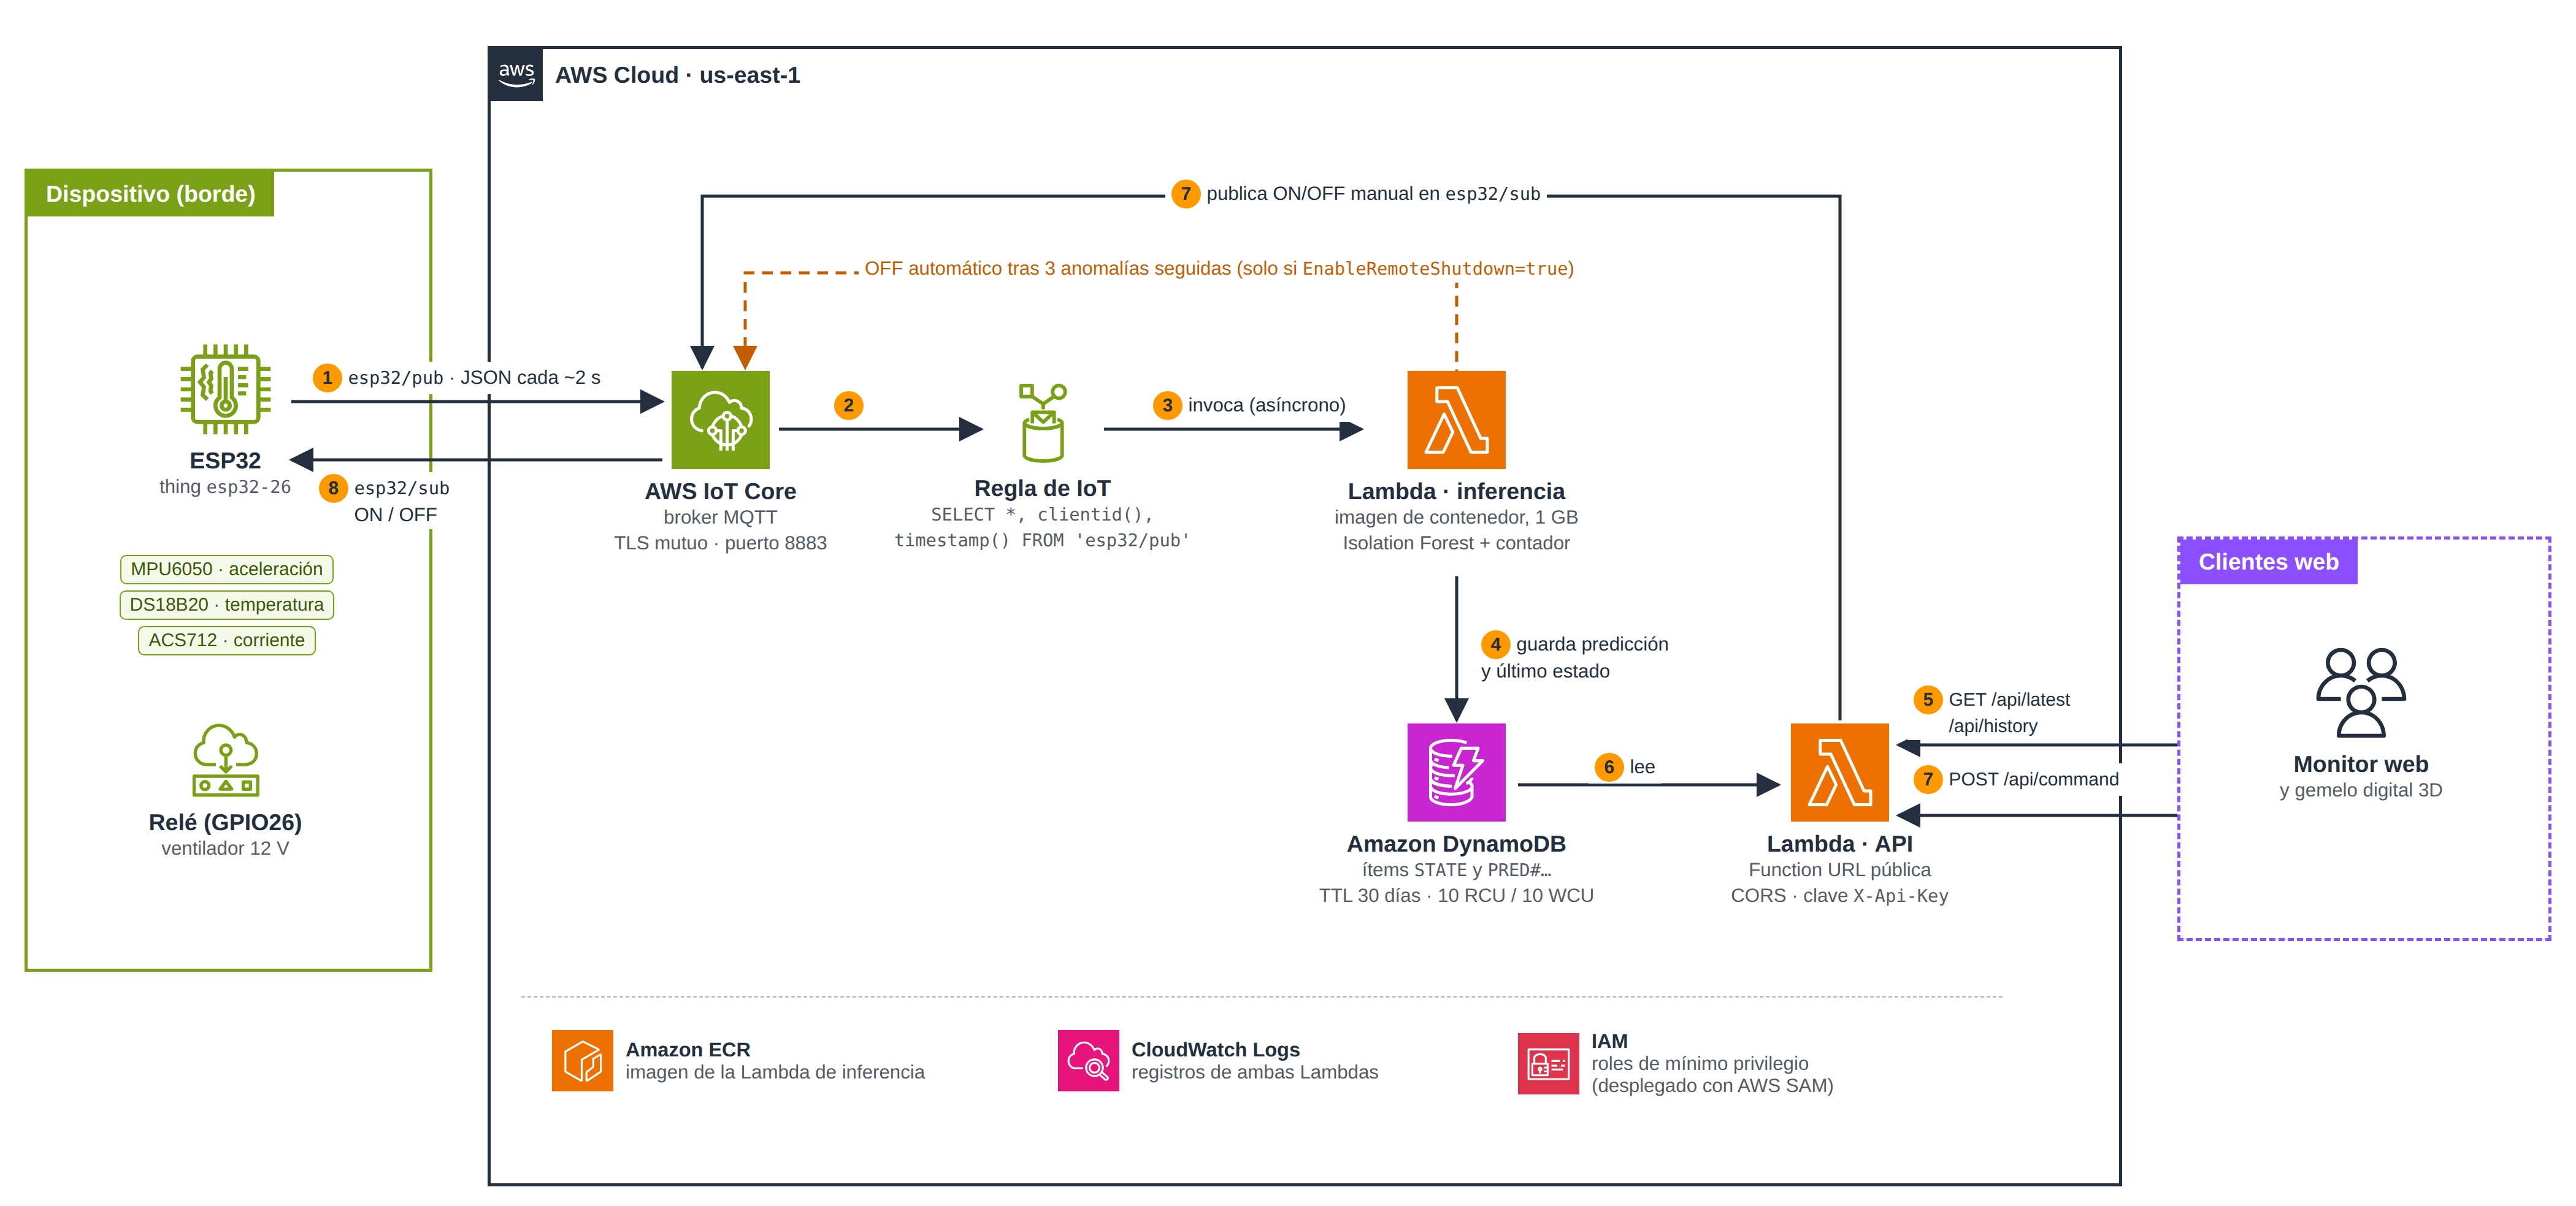
\includegraphics[width=\textwidth]{aws/arquitectura-aws.png}
\caption{Arquitectura del sistema en AWS. Pasos 1--4: adquisición e inferencia; pasos 5--8:
consulta y control desde el monitor web y el gemelo digital. La línea discontinua es la orden de
parada automática, desactivada en las pruebas.}
\label{fig:arq-aws}
\end{figure*}

\subsubsection{Infraestructura como código}
Toda la infraestructura se describe en una plantilla de AWS SAM (\code{template.yaml}) y se despliega
con \code{sam build} y \code{sam deploy}. La plantilla crea:
\begin{itemize}
  \item una \textbf{regla de IoT} con la consulta
        \code{SELECT *, clientid() AS client\_id, timestamp() AS received\_at FROM 'esp32/pub'},
        que añade al mensaje el identificador del cliente y la hora de recepción~\cite{awsrules};
  \item la \textbf{Lambda de inferencia}, empaquetada como imagen de contenedor en Amazon ECR
        (Python 3.12, 1\,024~MB, 30~s de tiempo máximo), porque scikit-learn, SciPy y pandas
        exceden el límite de 250~MB de un paquete comprimido~\cite{awslambda}. Como la regla la
        invoca de forma asíncrona, se desactivaron los reintentos y se descartan los eventos con más
        de 60~s en cola: una lectura vieja no sirve para decidir un apagado y un reintento podría
        contar dos veces la misma anomalía;
  \item la \textbf{Lambda de API}, un paquete comprimido de pocos kilobytes (Python 3.12, 256~MB)
        con una \emph{Function URL} pública y CORS habilitado, para que otra aplicación web la
        consuma directamente desde el navegador;
  \item una \textbf{tabla DynamoDB} con capacidad aprovisionada de 10 unidades de lectura y 10 de
        escritura, dentro de la capa gratuita, y expiración automática (TTL) de las predicciones a
        los 30 días;
  \item \textbf{roles IAM de mínimo privilegio}: la Lambda de inferencia solo escribe en la tabla y
        publica en \code{esp32/sub}; la de API solo lee la tabla y publica en \code{esp32/sub}.
\end{itemize}
Los parámetros de la plantilla permiten cambiar los tópicos, el número de anomalías consecutivas
(3 por defecto), la clave de los comandos manuales (\code{CommandApiKey}, que CloudFormation no
muestra) y habilitar o no el envío real de la orden de parada (\code{EnableRemoteShutdown},
desactivado por defecto hasta validar el sistema en banco). Con el dispositivo apagado no se generan
mensajes ni invocaciones, por lo que el costo en reposo es prácticamente nulo.

\subsubsection{Lógica de la Lambda de inferencia}
La Fig.~\ref{fig:flujo-lambda} muestra el procesamiento de cada mensaje. El modelo se carga una
sola vez por arranque en frío, por lo que las invocaciones siguientes solo ejecutan la inferencia.
Las lecturas con el ventilador apagado no pasan por el modelo, ya que se entrenó únicamente con
operación encendida, pero sí actualizan el estado del dispositivo y reinician el contador. Para cada
lectura válida, la función calcula $s=-\code{score\_samples}(x)$, que coincide con el puntaje de la
Ec.~\eqref{eq:iforest}, y su percentil frente a los puntajes de calibración. El contador de
anomalías consecutivas se actualiza de forma atómica en DynamoDB, de modo que dos invocaciones
simultáneas no pierden incrementos; es necesario guardarlo fuera de la función porque cada
invocación de Lambda es independiente y no conserva memoria de las anteriores.

\begin{figure}[H]
\centering
\begin{tikzpicture}[node distance=0.3cm]
  \node[inicio] (a) {Mensaje en \code{esp32/pub}};
  \node[proceso, below=of a] (b) {Regla IoT agrega \code{client\_id} y \code{received\_at}};
  \node[decision, below=of b] (c) {¿Estado ENCENDIDO?};
  \node[proceso, right=0.3cm of c, text width=1.5cm, minimum width=1.6cm] (c2) {Guardar estado\\contador = 0};
  \node[proceso, below=of c] (d) {Validar 5 variables\\$s=-\code{score\_samples}(x)$};
  \node[decision, below=of d] (e) {¿$s>$ umbral?};
  \node[proceso, right=0.3cm of e, text width=1.5cm, minimum width=1.6cm] (e2) {Contador = 0};
  \node[proceso, below=of e] (f) {Contador += 1 (atómico)};
  \node[decision, below=of f] (g) {¿Contador $\geq 3$?};
  \node[proceso, right=0.3cm of g, text width=1.5cm, minimum width=1.6cm] (g2) {Publicar OFF en \code{esp32/sub}\textsuperscript{*}};
  \node[proceso, below=of g] (h) {Guardar predicción y estado en DynamoDB};
  \node[inicio, below=of h] (z) {Fin};
  \draw[linea] (a) -- (b); \draw[linea] (b) -- (c);
  \draw[linea] (c) -- node[right, etiqueta]{sí} (d);
  \draw[linea] (c) -- node[above, etiqueta]{no} (c2);
  \draw[linea] (d) -- (e);
  \draw[linea] (e) -- node[right, etiqueta]{sí} (f);
  \draw[linea] (e) -- node[above, etiqueta]{no} (e2);
  \draw[linea] (e2.south) |- (h.east);
  \draw[linea] (f) -- (g);
  \draw[linea] (g) -- node[right, etiqueta]{no} (h);
  \draw[linea] (g) -- node[above, etiqueta]{sí} (g2);
  \draw[linea] (g2.south) |- ([yshift=3pt]h.east);
  \draw[linea] (h) -- (z);
\end{tikzpicture}
\caption{Diagrama de flujo de la Lambda de inferencia.
\textsuperscript{*}Solo si \code{EnableRemoteShutdown} está activo.}
\label{fig:flujo-lambda}
\end{figure}

\subsubsection{Modelo de datos en DynamoDB}
Todos los registros de un dispositivo comparten la clave de partición \code{DEVICE\#<id>} y se
distinguen por la clave de ordenamiento (Tabla~\ref{tab:dynamo}). Como esta empieza con la marca de
tiempo, las predicciones quedan ordenadas cronológicamente y las más recientes se obtienen con una
consulta, sin recorrer la tabla.

\begin{table}[H]
\centering
\caption{Ítems guardados por dispositivo en DynamoDB.}
\label{tab:dynamo}
\scriptsize
\begin{tabularx}{\columnwidth}{@{}>{\raggedright\arraybackslash}p{1.75cm}>{\raggedright\arraybackslash}X@{}}
\toprule
\textbf{Clave \code{sk}} & \textbf{Contenido} \\
\midrule
\code{STATE} & Un único ítem que se sobrescribe en cada lectura: contador de anomalías
consecutivas, estado del ventilador, última lectura y última predicción. Lo consulta el gemelo. \\
\code{PRED\#<ms>\#<id>} & Un ítem por lectura encendida: las 5 variables, \code{score}, umbral,
\code{is\_anomaly}, percentil, contador, \code{shutdown\_requested} y \code{shutdown\_sent}. Expira
a los 30 días. \\
\bottomrule
\end{tabularx}
\end{table}

\subsubsection{API para el monitor web y el gemelo digital}
La Lambda de API expone los recursos de la Tabla~\ref{tab:api}. Las lecturas son públicas y el
navegador puede consultarlas desde cualquier origen gracias a CORS. La orden manual exige la
cabecera \code{X-Api-Key}, que se compara en tiempo constante con la clave configurada; una
respuesta \code{202} indica que la orden se publicó, y la confirmación de que el relé conmutó llega
con la siguiente lectura en \code{/api/latest}.

\begin{table}[H]
\centering
\caption{Recursos de la API (\emph{Function URL}).}
\label{tab:api}
\scriptsize
\begin{tabularx}{\columnwidth}{@{}>{\raggedright\arraybackslash}p{2.35cm}>{\raggedright\arraybackslash}X@{}}
\toprule
\textbf{Recurso} & \textbf{Uso} \\
\midrule
\code{GET /api/latest} & Estado actual: \code{online} (lectura en los últimos 10~s), ventilador,
5 variables, predicción y contador. Una sola lectura de DynamoDB; pensado para consultarse cada
segundo desde el gemelo. \\
\code{GET /api/history} & Últimas $N$ predicciones ($1\le N\le 100$, por defecto 30), de la más
reciente a la más antigua. \\
\code{POST /api/command} & Cuerpo \code{\{"action":"ON"|"OFF"\}} con \code{X-Api-Key}; publica la
orden en \code{esp32/sub}. Sin clave válida responde \code{401}. \\
\bottomrule
\end{tabularx}
\end{table}

\subsubsection{Pruebas en AWS}
Las pruebas se hicieron con el prototipo conectado y publicando lecturas reales. En la consola de
DynamoDB (Fig.~\ref{fig:dynamo}) se observa que cada lectura genera un ítem de predicción, que el
contador de anomalías consecutivas crece de uno en uno y que \code{shutdown\_requested} pasa a
\code{true} al alcanzar la tercera anomalía, mientras \code{shutdown\_sent} permanece en
\code{false} porque el envío real estaba desactivado.

\begin{figure*}[t]
\centering
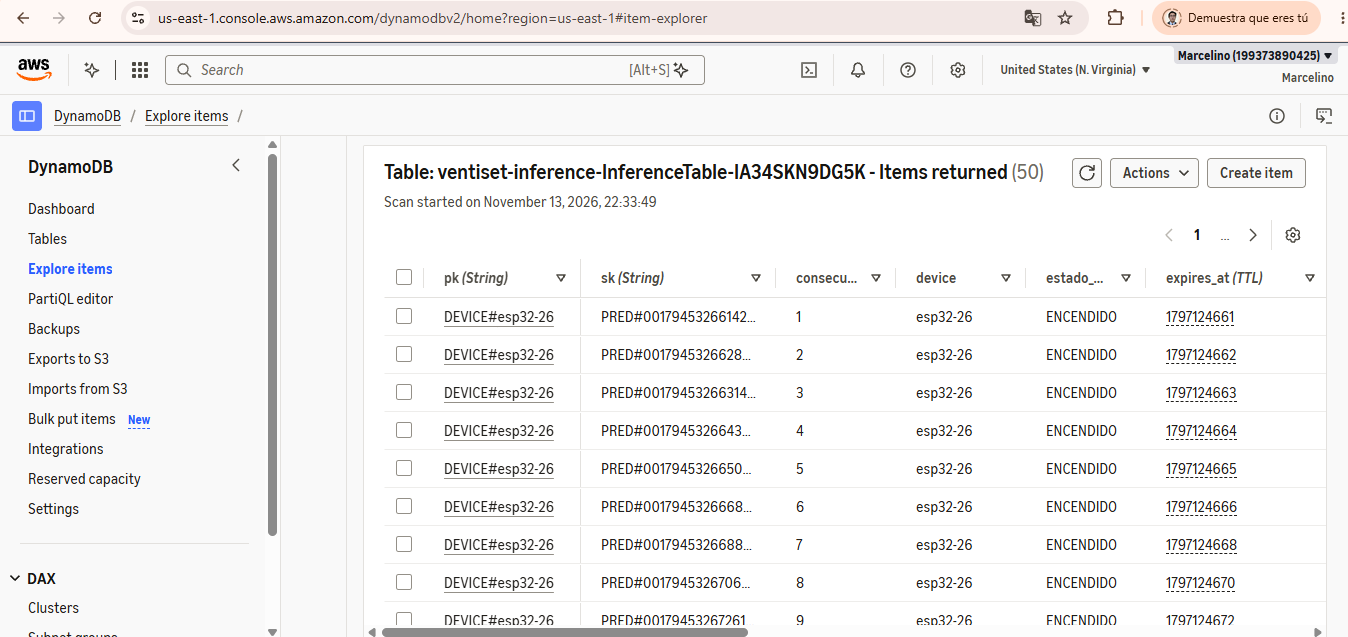
\includegraphics[width=0.49\textwidth]{aws/dynamodb-contador.png}\hfill
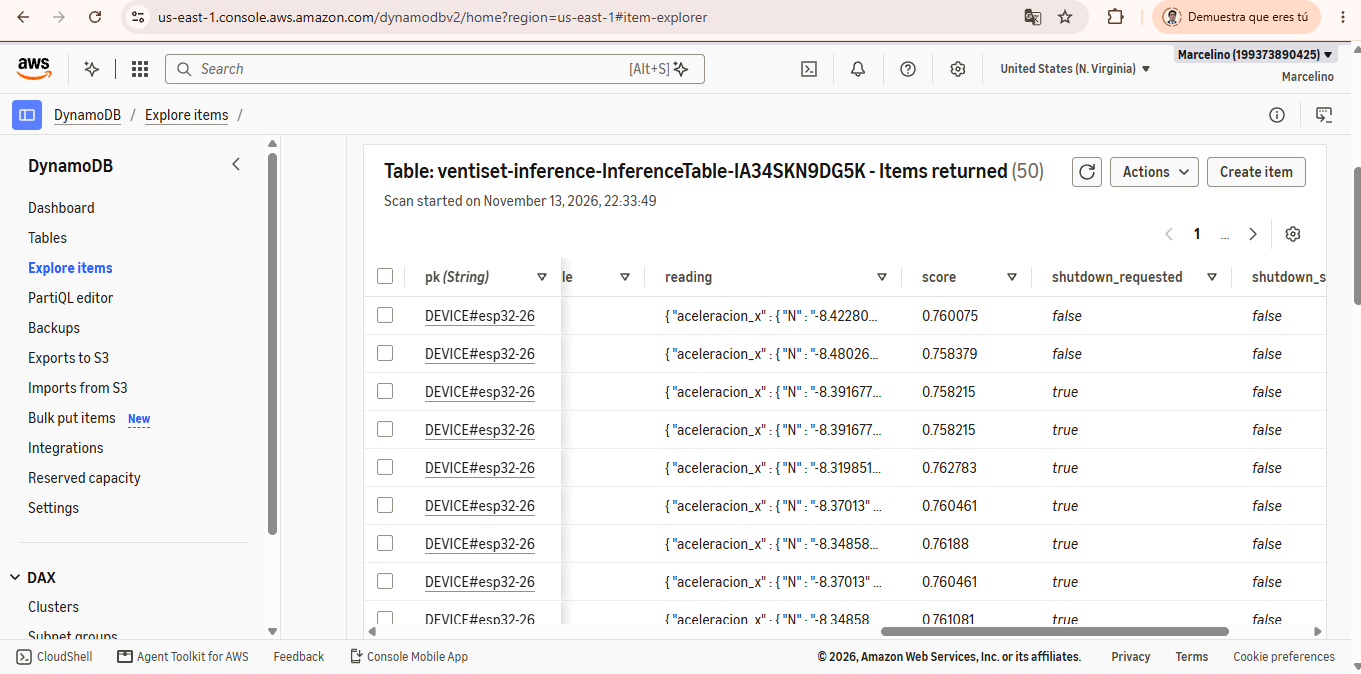
\includegraphics[width=0.49\textwidth]{aws/dynamodb-shutdown.png}
\caption{Ítems de predicción en la consola de DynamoDB. Izquierda: el contador
(\code{consecutive\_anomalies}) aumenta en cada lectura anómala. Derecha: \code{shutdown\_requested}
se activa desde la tercera anomalía; \code{shutdown\_sent} queda en \code{false} con
\code{EnableRemoteShutdown} desactivado.}
\label{fig:dynamo}
\end{figure*}

\begin{figure}[H]
\centering
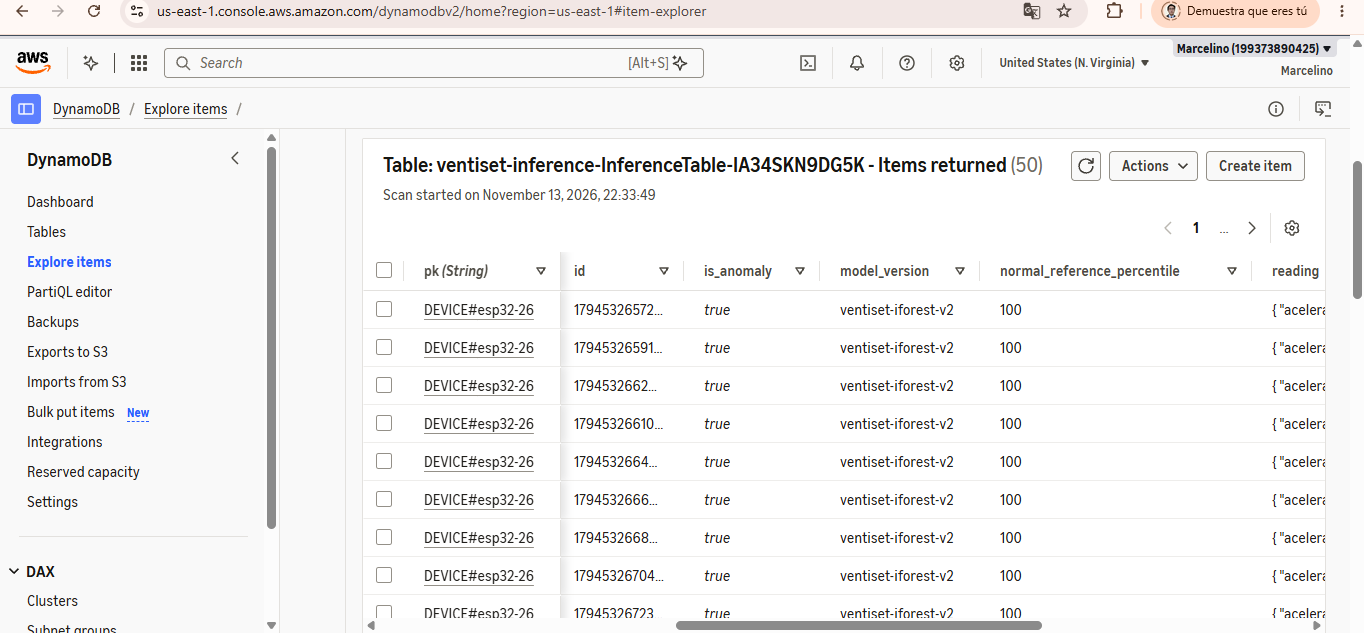
\includegraphics[width=\columnwidth]{aws/dynamodb-prediccion.png}
\caption{Resultado del modelo guardado en cada ítem: indicador de anomalía, versión del modelo,
percentil de referencia y la lectura original.}
\label{fig:dynamo-pred}
\end{figure}

La API se verificó con el dispositivo en línea. \code{/api/latest} devolvió el estado actual con una
antigüedad de 0.8--1.9~s respecto de la última lectura (Fig.~\ref{fig:api-latest}), y
\code{/api/history} devolvió las últimas 3 y 50 predicciones ordenadas por tiempo
(Figs.~\ref{fig:api-3} y \ref{fig:api-50}), con tiempos de respuesta de 10--121~ms desde el
navegador. Las 50 predicciones abarcan 92~s, es decir, el ESP32 publicó en promedio una lectura cada
${\sim}1.8$~s: el intervalo mínimo configurado es de 1~s, pero cada ciclo del firmware suma la
conversión del DS18B20, el promedio de 64 muestras del ACS712 y una pausa de 300~ms, por lo que la
publicación ocurre en el ciclo siguiente a cumplirse ese intervalo. La petición \code{POST /api/command} sin clave fue rechazada
con \code{401}. Con la clave correcta se ejecutaron tres ciclos \code{OFF}/\code{ON}: la API
respondió \code{202} en 0.48--0.93~s y el cambio de estado se confirmó en \code{/api/latest} en
3.6--7.2~s para \code{OFF} (media 5.3~s) y en 3.7--4.1~s para \code{ON} (media 3.9~s). Este tiempo
es una cota superior de la conmutación del relé, porque incluye esperar la siguiente lectura del
ESP32 y su paso por la Lambda de inferencia. La mayor parte se debe a que el firmware atiende los
mensajes MQTT una vez por ciclo de ${\sim}1.8$~s, por lo que una orden puede esperar casi un ciclo
completo antes de ejecutarse. Además, el firmware no guarda la última orden recibida: si el ESP32 se
reinicia después de un \code{OFF}, el ventilador vuelve a encenderse en \code{setup()}.

\begin{figure}[H]
\centering
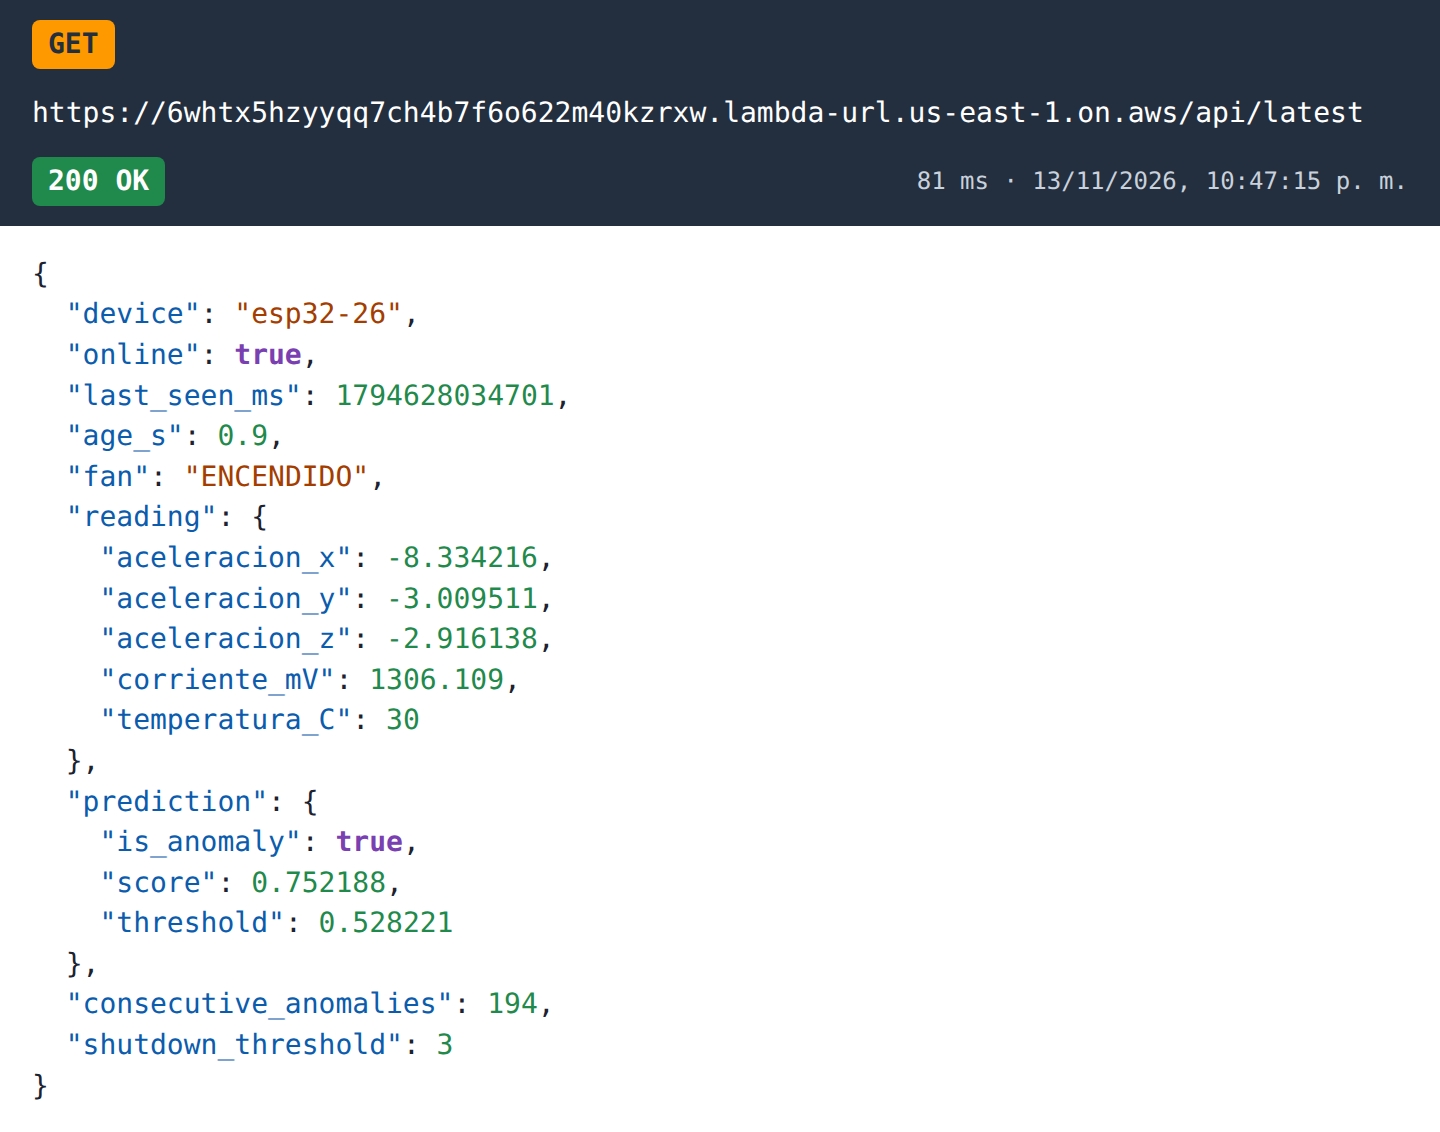
\includegraphics[width=0.82\columnwidth]{aws/api-latest.png}
\caption{Respuesta de \code{GET /api/latest} con el ESP32 en línea.}
\label{fig:api-latest}
\end{figure}

\begin{figure}[H]
\centering
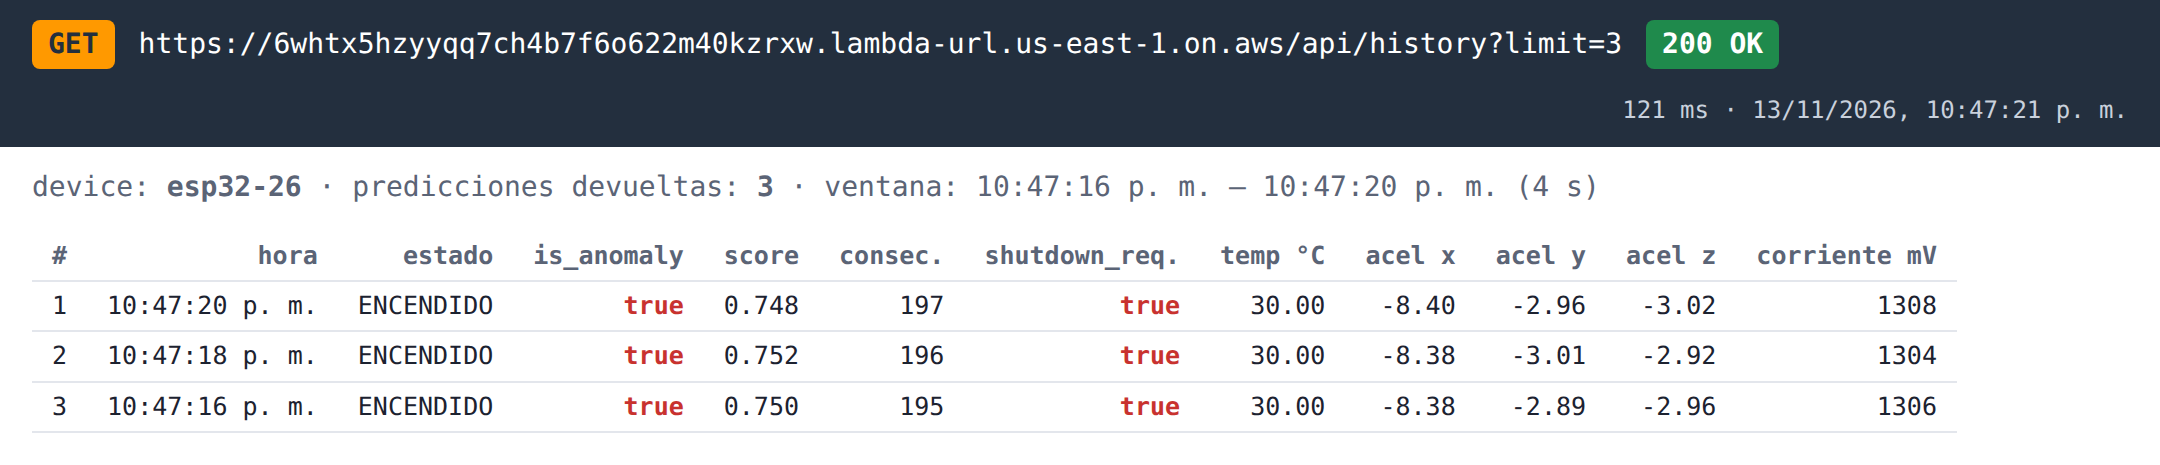
\includegraphics[width=\columnwidth]{aws/api-history-3.png}
\caption{Últimas 3 predicciones (\code{GET /api/history?limit=3}).}
\label{fig:api-3}
\end{figure}

\begin{figure}[H]
\centering
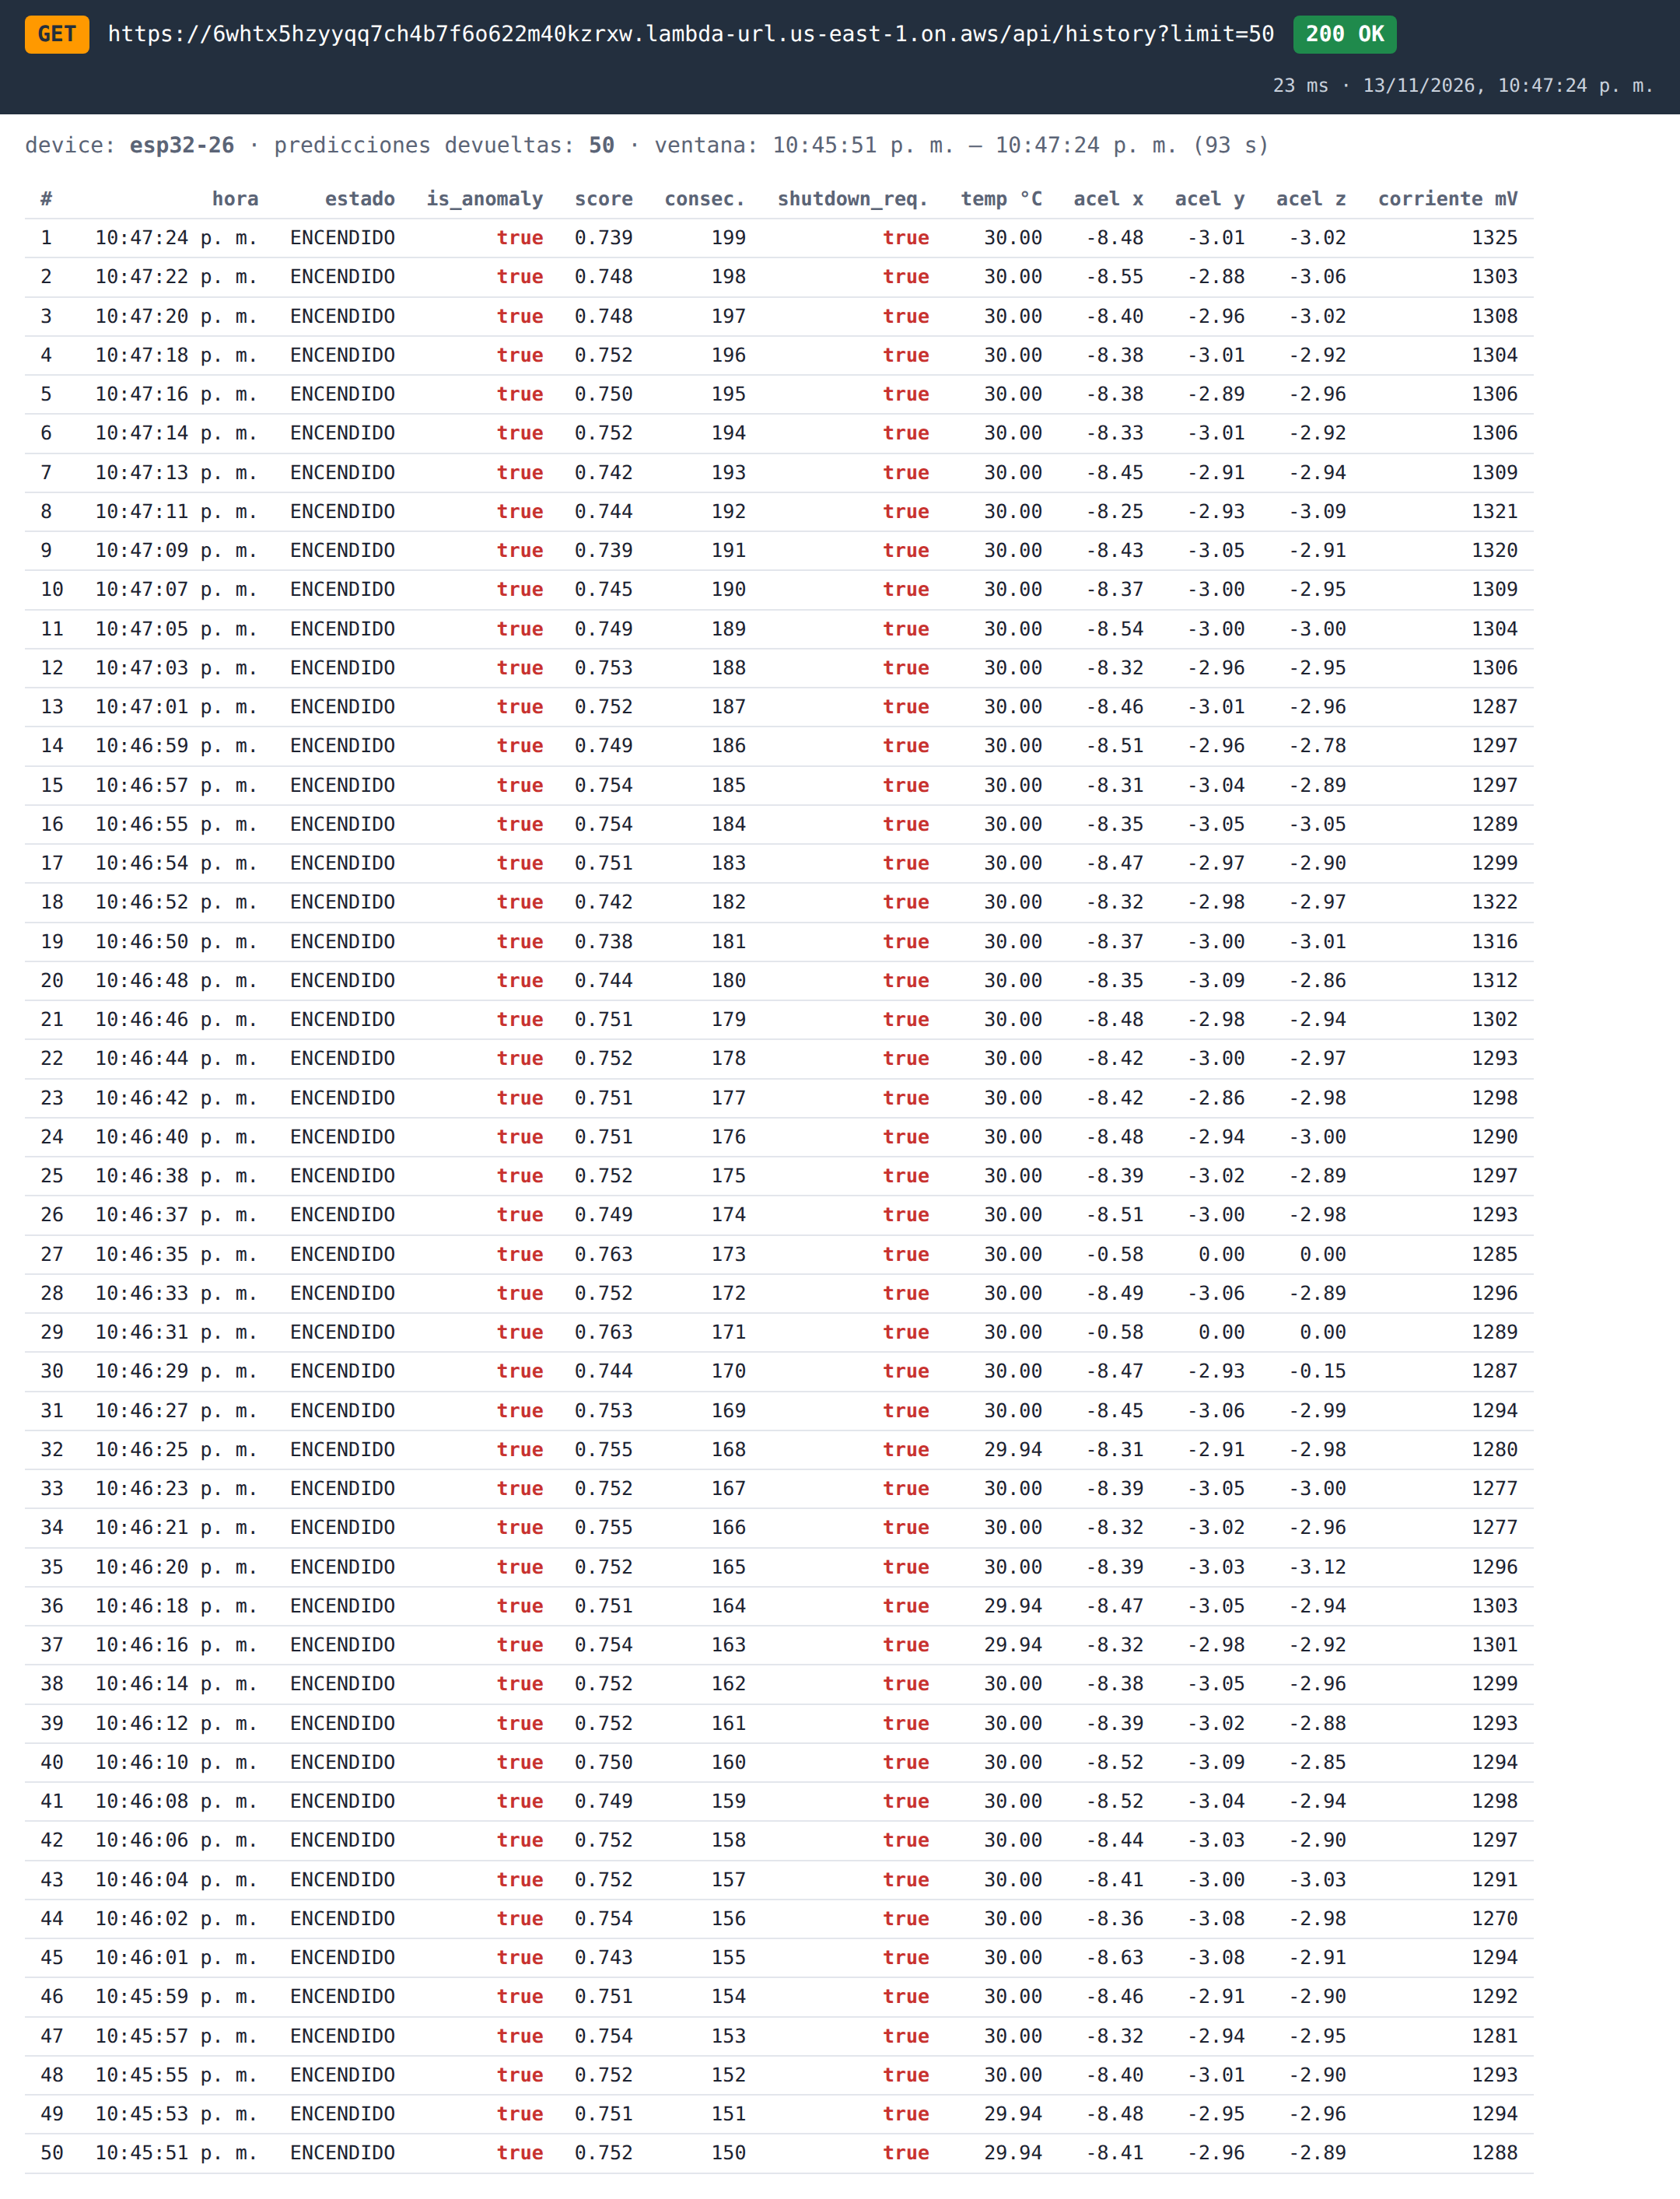
\includegraphics[width=\columnwidth,height=11cm,keepaspectratio]{aws/api-history-50.png}
\caption{Últimas 50 predicciones (\code{GET /api/history?limit=50}), la ventana que consume el
gemelo digital para sus gráficos.}
\label{fig:api-50}
\end{figure}

Sobre esta API se construyó un monitor web de prueba (Fig.~\ref{fig:web}) que reproduce lo que hará
el gemelo digital: consulta \code{/api/latest} cada segundo y \code{/api/history} cada 5~s, muestra
el estado del ventilador, las cinco variables y su evolución, y permite enviar \code{ON} y
\code{OFF}.

\begin{figure}[H]
\centering
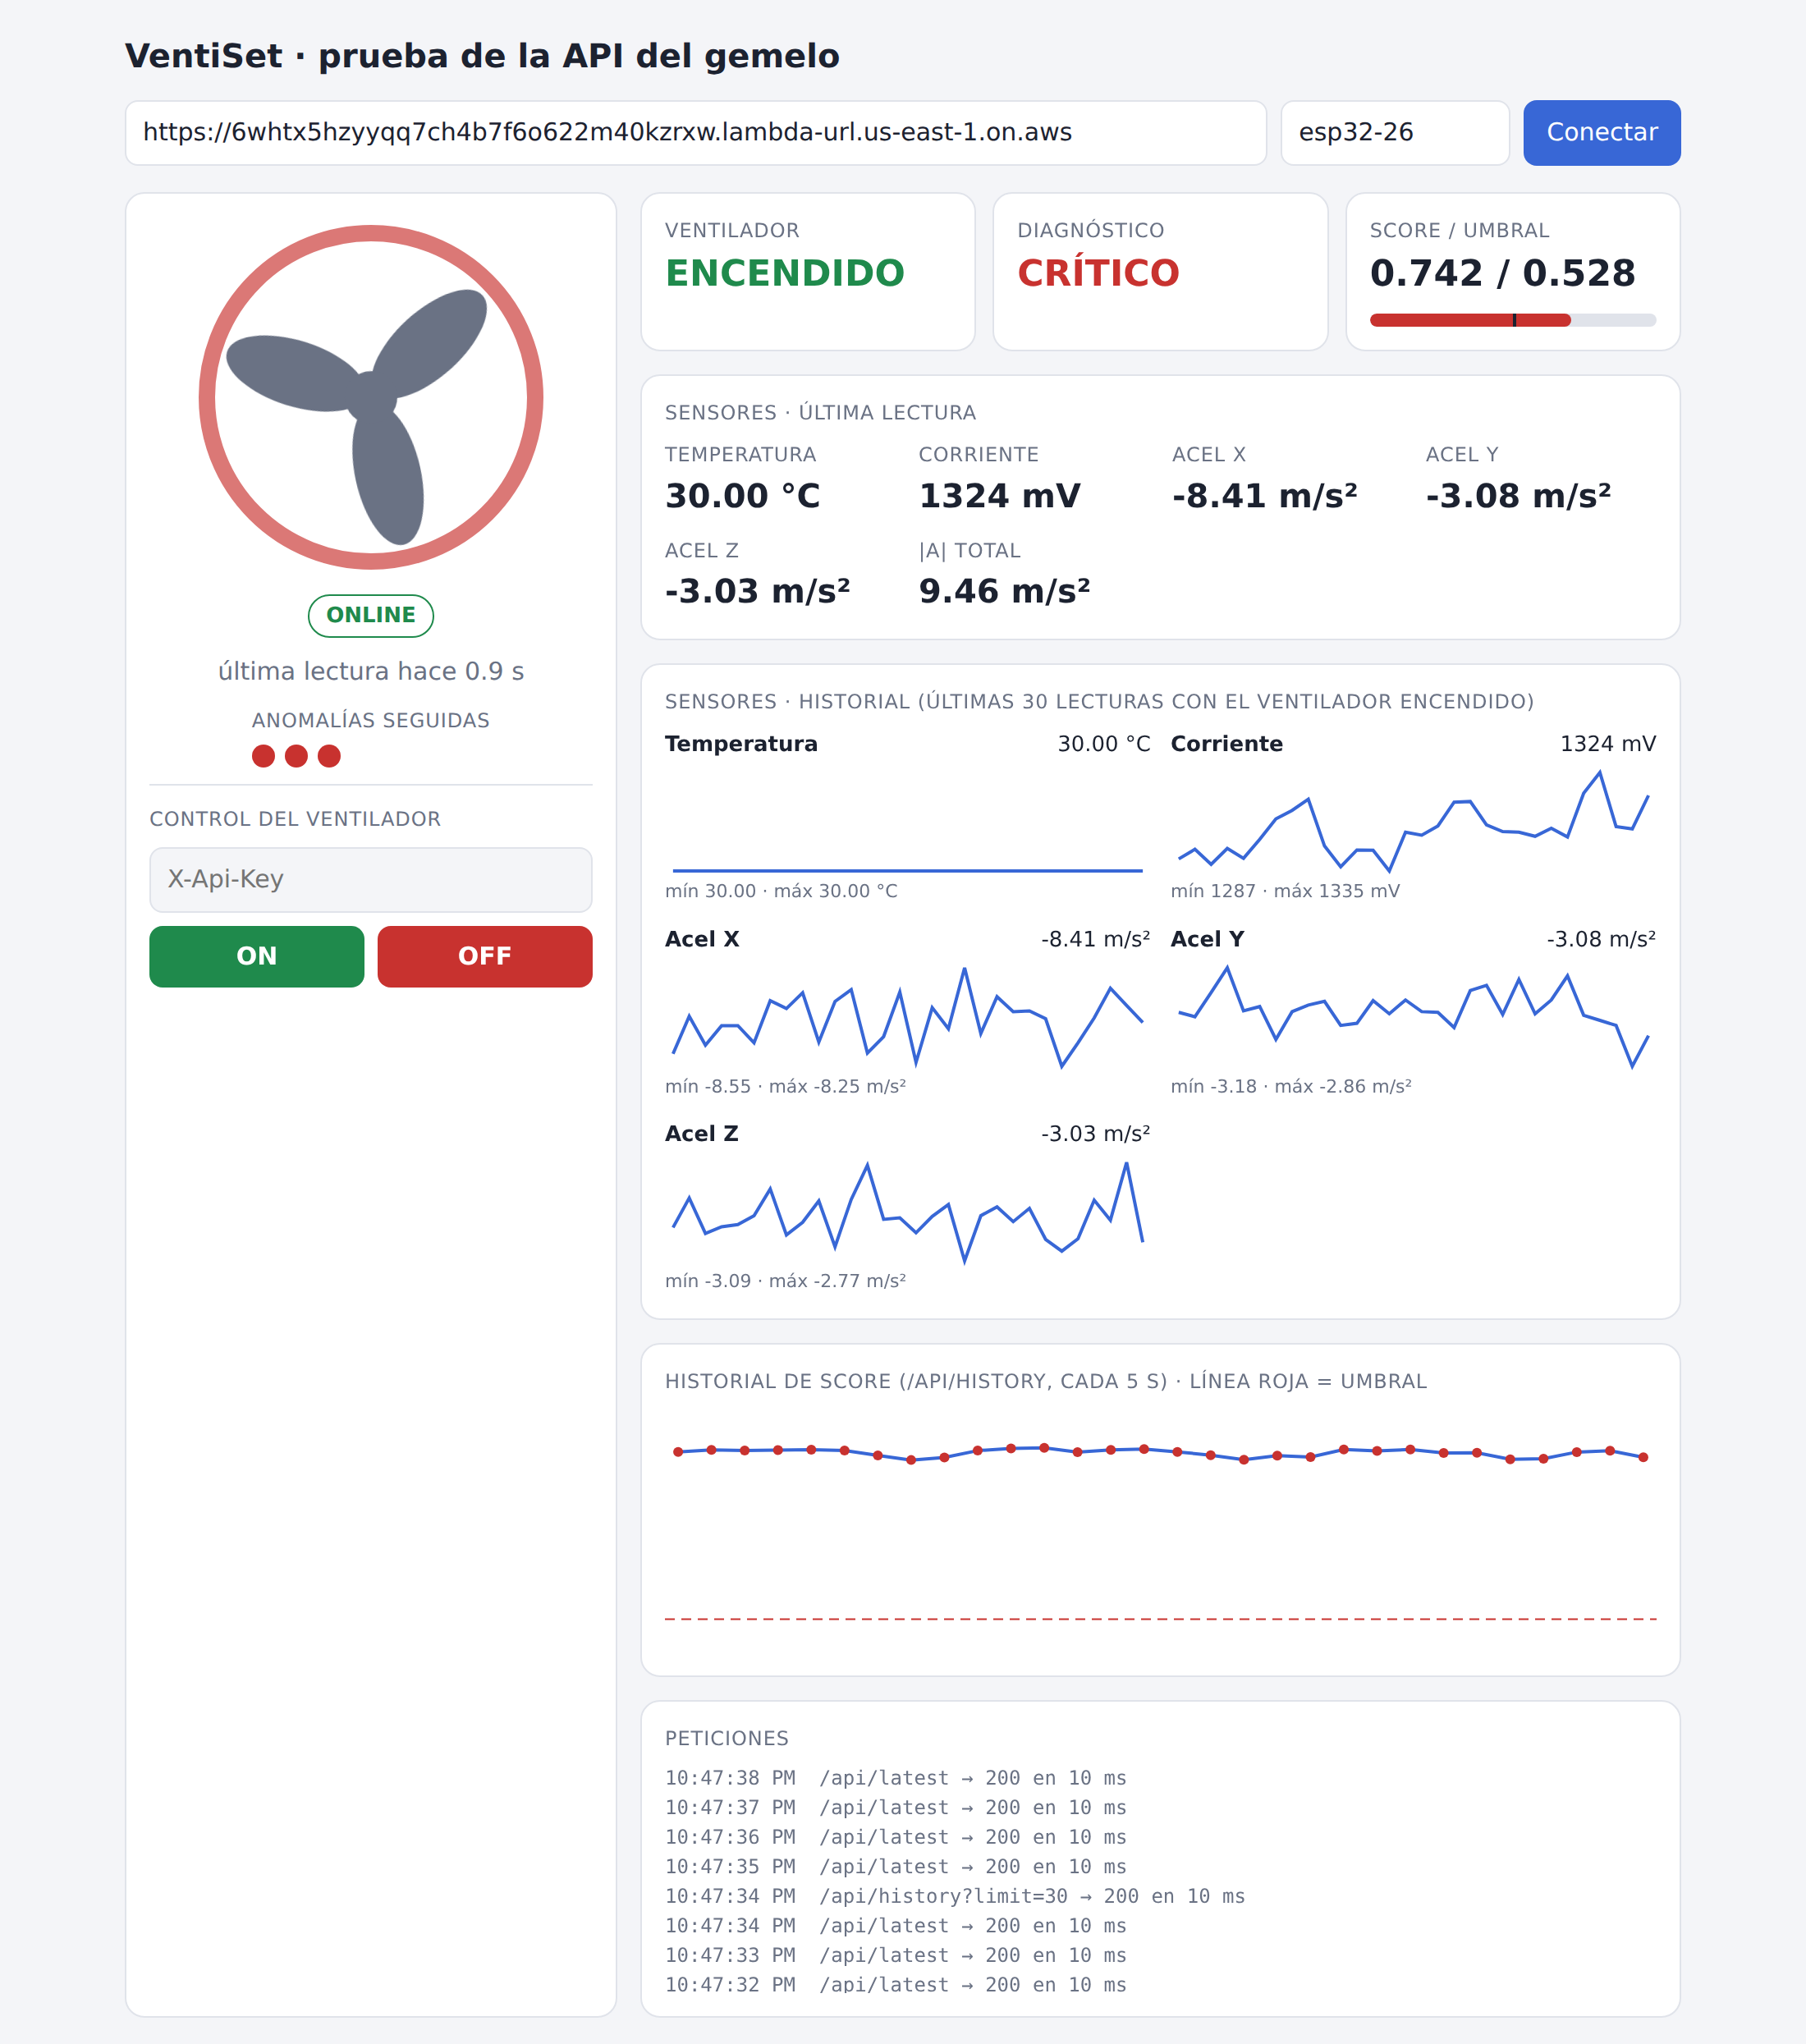
\includegraphics[width=\columnwidth]{aws/web-gemelo.png}
\caption{Monitor web consumiendo la API con el dispositivo en línea. El estado crítico corresponde
a la secuencia de anomalías discutida en el texto.}
\label{fig:web}
\end{figure}

Todas las lecturas de esta sesión se marcaron como anómalas ($s\approx0.75$ frente a un umbral de
0.528, percentil~100), y el contador superó las 190 anomalías consecutivas. La causa no está en la
cadena IoT sino en los datos: frente al conjunto de entrenamiento, el acelerómetro quedó montado con
otra orientación (eje $y\approx-3$ y eje $z\approx-3$~m/s$^2$, frente a ${\approx}0$ y
${\approx}4$~m/s$^2$) y la temperatura del motor estaba 4~°C más alta. El detector reconoce
correctamente que estas lecturas no se parecen a la operación con la que se entrenó, pero el
resultado confirma que la orden de parada automática no debe habilitarse hasta reentrenar el modelo
con el montaje definitivo (Sección~\ref{sec:discusion}).

\subsection{Recorrido guiado por el sitio web VentiSet}
\label{sec:recorrido-web}

El sitio web reúne en un solo recorrido la presentación del prototipo, su simulador, los datos,
el modelo, la evaluación, la nube y las limitaciones. La Fig.~\ref{fig:web-recorrido} resume el
orden de navegación documentado en las capturas. Estas pantallas son evidencia de la interfaz y
de los escenarios que muestra; no constituyen por sí solas una nueva medición experimental. En
particular, se distinguen el banco simulado, la reproducción de filas históricas de
\code{VentiSet.csv} y las pruebas del prototipo físico descritas en la Sección~\ref{sec:resultados}.

\begin{figure*}[t]
\centering
\resizebox{\textwidth}{!}{%
\begin{tikzpicture}[node distance=0.22cm]
  \node[bloque, text width=2.3cm, minimum height=1.15cm] (w1)
    {\textbf{01 · Inicio}\\Propósito y alcance};
  \node[bloque, text width=2.3cm, minimum height=1.15cm, right=of w1] (w2)
    {\textbf{02--06 · Simulador}\\Normal, OFF preparado y enviado};
  \node[nucleo, text width=2.3cm, minimum height=1.15cm, right=of w2] (w3)
    {\textbf{07--08 · Datos}\\Montaje y señales};
  \node[nucleo, text width=2.3cm, minimum height=1.15cm, right=of w3] (w4)
    {\textbf{09--10 · Modelo}\\Isolation Forest y selección};
  \node[nucleo, text width=2.3cm, minimum height=1.15cm, right=of w4] (w5)
    {\textbf{11--12 · Evaluación}\\Prueba, ruido y PCA};
  \node[bloque, text width=2.3cm, minimum height=1.15cm, right=of w5] (w6)
    {\textbf{13 · Nube}\\Mensajes e inferencia};
  \node[actuador, text width=2.3cm, minimum height=1.15cm, right=of w6] (w7)
    {\textbf{14 · Límites}\\Alcance y trabajo pendiente};
  \foreach \a/\b in {w1/w2,w2/w3,w3/w4,w4/w5,w5/w6,w6/w7}
    \draw[flecha] (\a) -- (\b);
\end{tikzpicture}%
}
\caption{Flujo de navegación por las vistas documentadas del sitio VentiSet.}
\label{fig:web-recorrido}
\end{figure*}

La portada (captura~01) sintetiza el prototipo, los resultados principales y lo que aún falta
validar. El simulador permite observar primero un estado de referencia con puntaje 0.378, por
debajo del umbral 0.5282 (captura~02); luego, al activar el desplazamiento del MPU6050, muestra
anomalías consecutivas y una orden OFF preparada, pero no enviada cuando
\code{EnableRemoteShutdown} está desactivado (captura~03). La captura~04 presenta el escenario
separado con el envío habilitado: la pestaña Lambda registra la decisión y el ítem \code{STATE}
aparece como \code{APAGADO}. Este recorrido permite explicar la regla de persistencia; la
conmutación física del relé se sustenta en las pruebas de la Tabla~\ref{tab:funcional}, no solo en
la animación del simulador.

\begin{figure*}[t]
\centering
\begin{minipage}[t]{0.485\textwidth}
  \centering
  \includegraphics[width=\linewidth]{imagenes/recorrido-web/01-inicio.png}\\[-2pt]
  {\scriptsize (a) Inicio: objetivo, resultados y pendientes.\par}
\end{minipage}\hfill
\begin{minipage}[t]{0.485\textwidth}
  \centering
  \includegraphics[width=\linewidth]{imagenes/recorrido-web/02-simulador-normal.png}\\[-2pt]
  {\scriptsize (b) Banco simulado en estado habitual: $s=0.378<0.5282$.\par}
\end{minipage}

\vspace{0.25cm}

\begin{minipage}[t]{0.485\textwidth}
  \centering
  \includegraphics[width=\linewidth]{imagenes/recorrido-web/03-simulador-off-preparado.png}\\[-2pt]
  {\scriptsize (c) Tres o más anomalías: OFF preparado, con envío remoto deshabilitado.\par}
\end{minipage}\hfill
\begin{minipage}[t]{0.485\textwidth}
  \centering
  \includegraphics[width=\linewidth]{imagenes/recorrido-web/04-simulador-off-enviado-lambda.png}\\[-2pt]
  {\scriptsize (d) Escenario con envío habilitado: decisión Lambda y estado OFF.\par}
\end{minipage}
\caption{Inicio y escenarios guiados del simulador. Los estados preparado y enviado son dos
configuraciones distintas de la demostración.}
\label{fig:web-simulador}
\end{figure*}

La pestaña MQTT (captura~05) hace visibles los mensajes de \code{esp32/pub}, los resultados en
\code{ventiset/inference/esp32-26} y las órdenes en \code{esp32/sub}, conectando la interfaz con
la arquitectura descrita en la Sección~\ref{sec:implementacion}. En modo «Sesión real», la
captura~06 reproduce filas ordenadas de \code{VentiSet.csv} por la misma ruta de procesamiento;
es una reproducción de datos históricos, no una nueva adquisición en vivo. La sección Datos
documenta el montaje y las lecturas serie (captura~07), y luego presenta las cinco señales de las
3\,927 filas seleccionadas, incluido el tramo de reubicación del acelerómetro (captura~08).

\begin{figure*}[t]
\centering
\begin{minipage}[t]{0.485\textwidth}
  \centering
  \includegraphics[width=\linewidth]{imagenes/recorrido-web/05-simulador-mqtt.png}\\[-2pt]
  {\scriptsize (a) Tráfico observado en los tópicos MQTT.\par}
\end{minipage}\hfill
\begin{minipage}[t]{0.485\textwidth}
  \centering
  \includegraphics[width=\linewidth]{imagenes/recorrido-web/06-simulador-sesion-real.png}\\[-2pt]
  {\scriptsize (b) Reproducción ordenada de registros de VentiSet.csv.\par}
\end{minipage}

\vspace{0.25cm}

\begin{minipage}[t]{0.485\textwidth}
  \centering
  \includegraphics[width=\linewidth]{imagenes/recorrido-web/07-datos.png}\\[-2pt]
  {\scriptsize (c) Evidencia del montaje físico y el monitor serie.\par}
\end{minipage}\hfill
\begin{minipage}[t]{0.485\textwidth}
  \centering
  \includegraphics[width=\linewidth]{imagenes/recorrido-web/08-datos-senales.png}\\[-2pt]
  {\scriptsize (d) Señales registradas y reubicación del MPU6050.\par}
\end{minipage}
\caption{Del transporte de mensajes a la inspección del conjunto de datos y la evidencia física.}
\label{fig:web-datos}
\end{figure*}

La vista del modelo (captura~09) ilustra la lógica de Isolation Forest comparando dos lecturas
del conjunto: una típica requiere en promedio 12.7 cortes para aislarse y una del tramo de
reubicación, 3.4, en los 400 árboles del modelo elegido. La captura~10 muestra la búsqueda de
12 configuraciones y destaca la número~12 (FPR 1.02\,\%, utilidad $U=0.810$ y detección
sintética 83.1\,\%). La vista de evaluación separa las 590 lecturas de prueba, de las que 7
(1.19\,\%) superaron el umbral, de la reproducción de la sesión completa usada para mostrar
dónde se habría preparado una orden por persistencia (captura~11). Son análisis distintos: las
lecturas finales no participan en el ajuste, y las marcas no son etiquetas de fallas reales.
La captura~12 reúne las curvas de perturbación sintética de 0 a 100\,\% y la trayectoria de una
lectura en la proyección PCA; ambas visualizaciones describen el experimento de sensibilidad, no
una severidad física de falla.

\begin{figure*}[t]
\centering
\begin{minipage}[t]{0.485\textwidth}
  \centering
  \includegraphics[width=\linewidth]{imagenes/recorrido-web/09-modelo-aislamiento.png}\\[-2pt]
  {\scriptsize (a) Ejemplo de aislamiento en el bosque entrenado.\par}
\end{minipage}\hfill
\begin{minipage}[t]{0.485\textwidth}
  \centering
  \includegraphics[width=\linewidth]{imagenes/recorrido-web/10-modelo-hiperparametros.png}\\[-2pt]
  {\scriptsize (b) Comparación de las 12 configuraciones.\par}
\end{minipage}

\vspace{0.25cm}

\begin{minipage}[t]{0.485\textwidth}
  \centering
  \includegraphics[width=\linewidth]{imagenes/recorrido-web/11-evaluacion-prueba.png}\\[-2pt]
  {\scriptsize (c) Bloque de prueba y análisis temporal de persistencia.\par}
\end{minipage}\hfill
\begin{minipage}[t]{0.485\textwidth}
  \centering
  \includegraphics[width=\linewidth]{imagenes/recorrido-web/12-evaluacion-ruido-pca.png}\\[-2pt]
  {\scriptsize (d) Perturbación progresiva y proyección PCA.\par}
\end{minipage}
\caption{Vistas del modelo y la evaluación. El resultado sintético no equivale a sensibilidad
ante fallas físicas.}
\label{fig:web-modelo-evaluacion}
\end{figure*}

La vista Nube (captura~13) sigue el JSON desde \code{esp32/pub}, muestra los campos que agrega la
regla de IoT y la respuesta de Lambda, y relaciona la predicción con el estado almacenado en
DynamoDB y el canal de retorno. Estos elementos corresponden a la arquitectura y pruebas AWS ya
descritas; la captura no cambia el alcance de validación establecido allí. Finalmente, la vista
Límites (captura~14) cierra el recorrido separando lo implementado de lo que requiere nuevos
ensayos: mayor frecuencia de muestreo, fallas etiquetadas, más sesiones, calibración del ACS712 y
protección local independiente de la nube.

\begin{figure*}[t]
\centering
\begin{minipage}[t]{0.485\textwidth}
  \centering
  \includegraphics[width=\linewidth]{imagenes/recorrido-web/13-nube.png}\\[-2pt]
  {\scriptsize (a) Recorrido del mensaje y la respuesta por la nube AWS.\par}
\end{minipage}\hfill
\begin{minipage}[t]{0.485\textwidth}
  \centering
  \includegraphics[width=\linewidth]{imagenes/recorrido-web/14-limites.png}\\[-2pt]
  {\scriptsize (b) Límites conocidos y siguientes pasos experimentales.\par}
\end{minipage}
\caption{Cierre del recorrido: integración en la nube y delimitación del alcance experimental.}
\label{fig:web-nube-limites}
\end{figure*}

\section{Análisis de resultados}
\label{sec:resultados}

\subsection{Adquisición y calidad de las señales}

La Fig.~\ref{fig:senales} muestra las cinco señales del conjunto VentiSet con el ventilador
encendido. El periodo mediano entre lecturas fue de 0.94~s (cerca de 1.07~Hz). Lo fijan la conversión de 12~bits del DS18B20 (hasta 750~ms~\cite{ds18b20}), el promedio
de 64 muestras del ACS712 y la espera de 300~ms del bucle. La Tabla~\ref{tab:estadisticos} resume las estadísticas descriptivas tras excluir los
primeros 60 registros encendidos.

\begin{figure*}[t]
\centering
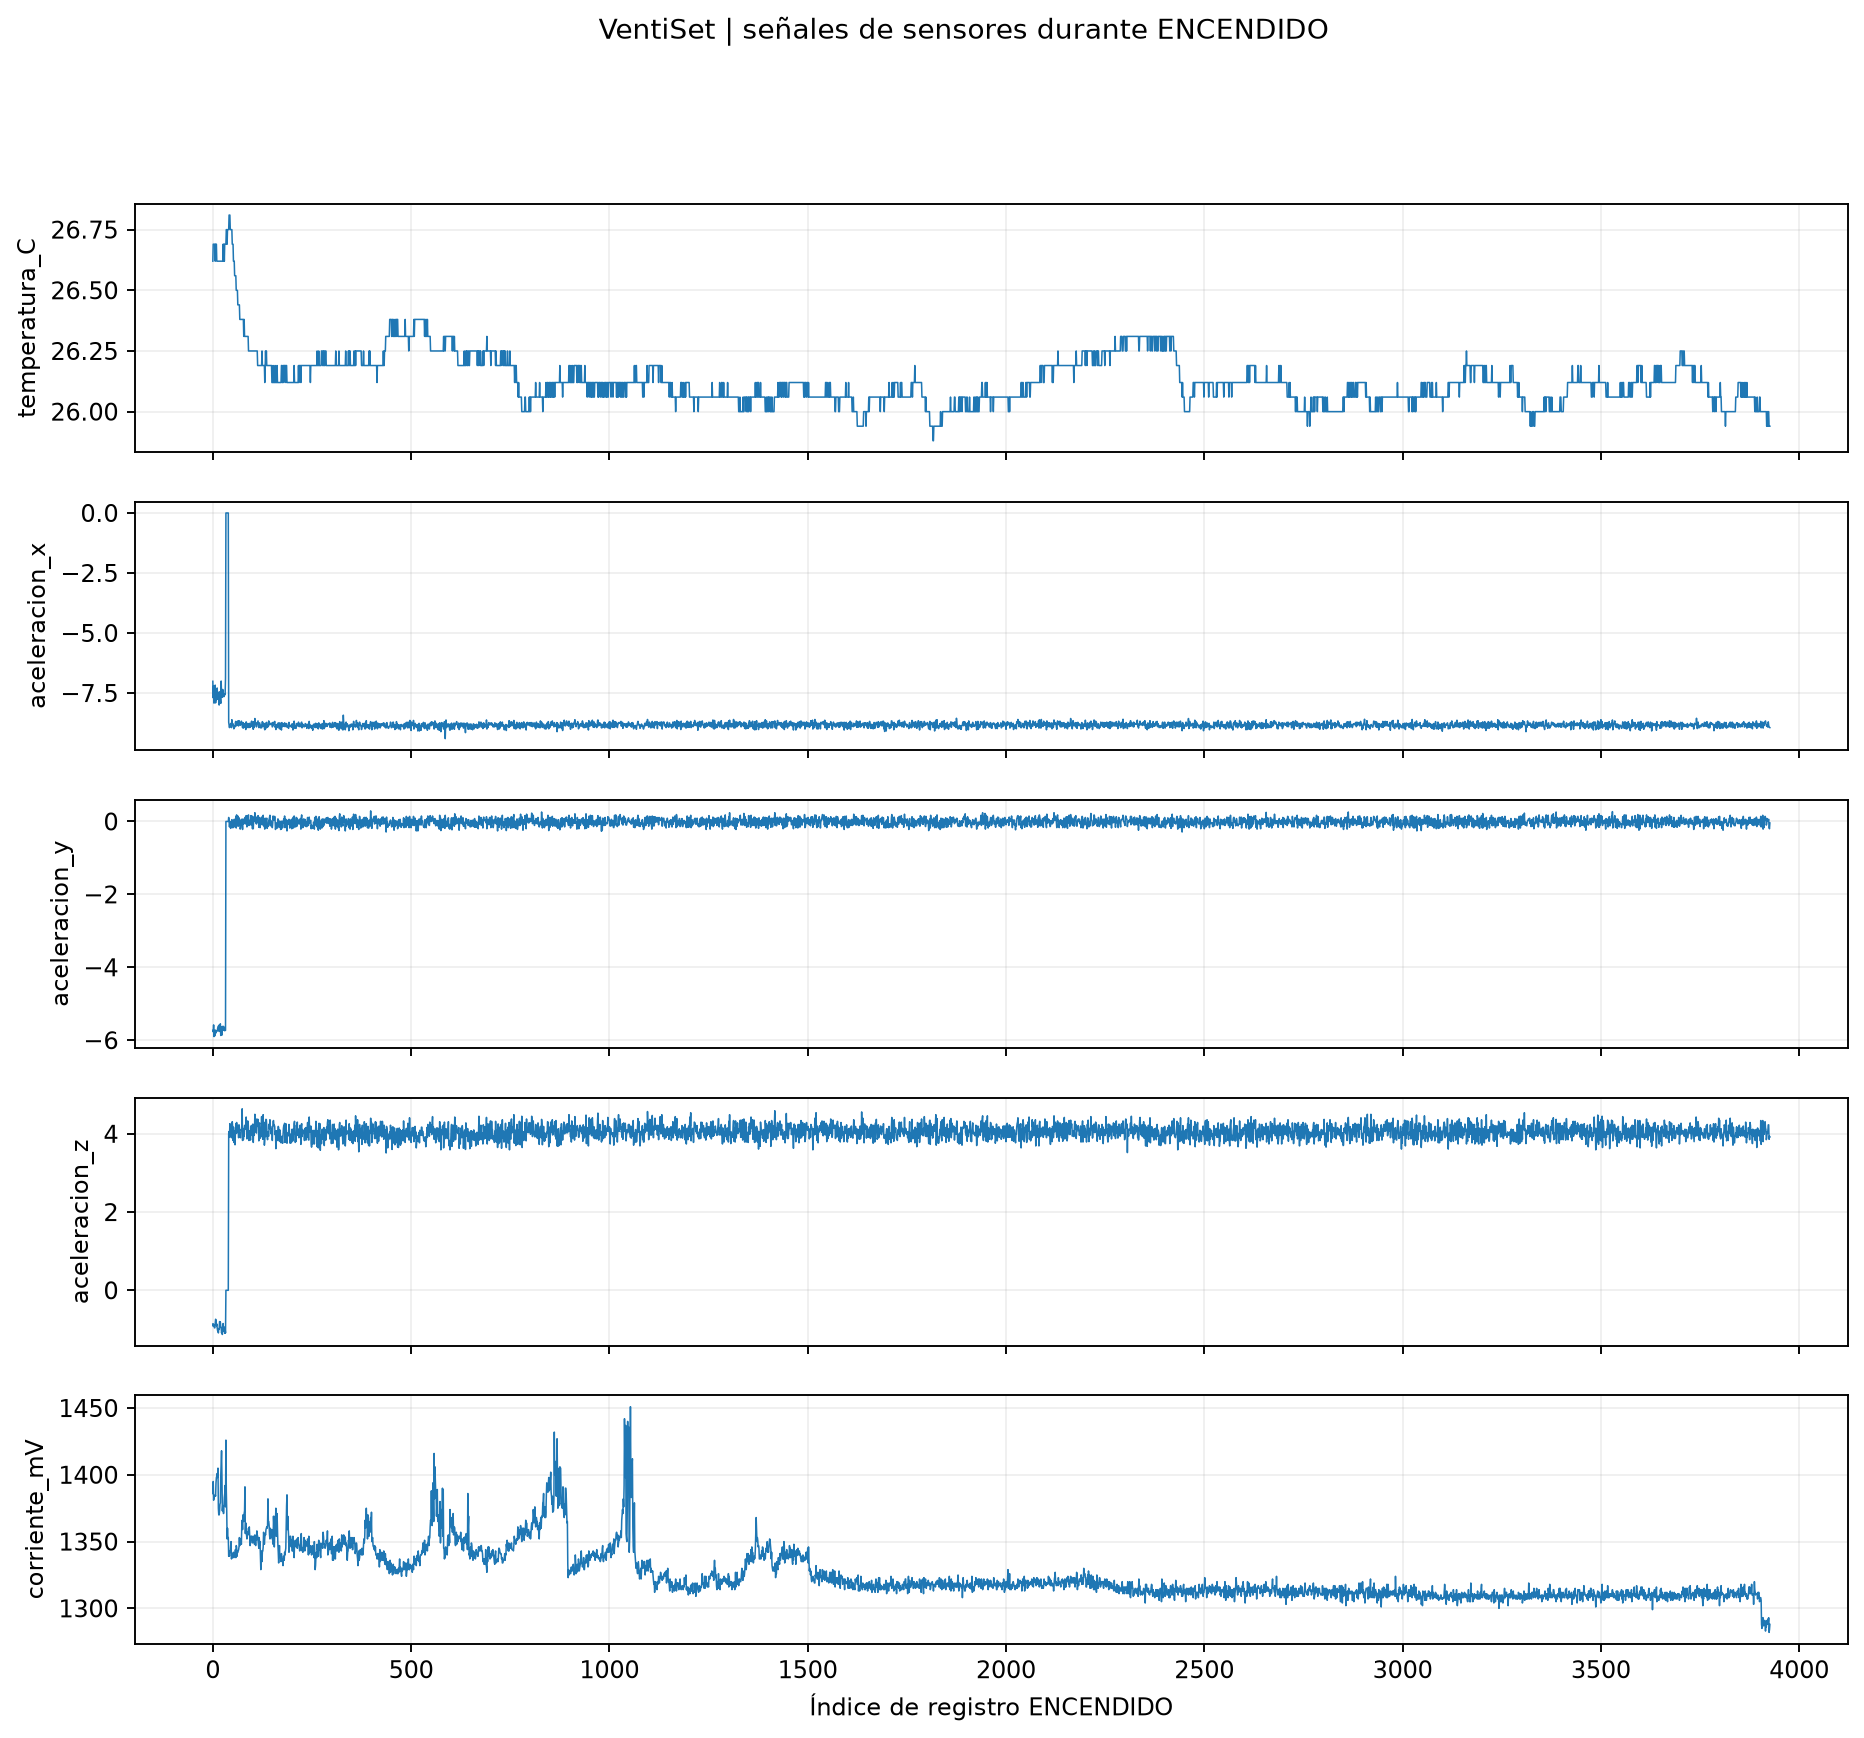
\includegraphics[width=0.92\textwidth,height=9.5cm,keepaspectratio]{imagenes/resultados/01_senales.png}
\caption{Señales registradas con el ventilador encendido (3\,927 lecturas, 69~min). De arriba
abajo: temperatura (°C), aceleración en X, Y y Z (m/s$^2$) y tensión del ACS712 (mV). Figura
generada por el equipo a partir de VentiSet.}
\label{fig:senales}
\end{figure*}

\begin{table}[htbp]
\centering
\caption{Estadísticas de las señales en régimen estable.}
\label{tab:estadisticos}
\footnotesize
\begin{tabular}{@{}lrrrr@{}}
\toprule
\textbf{Variable} & \textbf{Media} & \textbf{Desv.} & \textbf{Mín.} & \textbf{Máx.} \\
\midrule
Temperatura (°C) & 26.12 & 0.09 & 25.88 & 26.50 \\
$a_x$ (m/s$^2$) & $-8.83$ & 0.09 & $-9.40$ & $-8.42$ \\
$a_y$ (m/s$^2$) & $-0.01$ & 0.10 & $-0.29$ & 0.29 \\
$a_z$ (m/s$^2$) & 4.05 & 0.17 & 3.51 & 4.64 \\
ACS712 (mV) & 1\,324.6 & 19.2 & 1\,282 & 1\,451 \\
\bottomrule
\end{tabular}
\end{table}

Se observan tres hechos. Primero, en los primeros ${\sim}40$ registros la aceleración cambia
bruscamente de nivel en los tres ejes: el sensor se reubicó tras uno de los reinicios y el vector
de gravedad quedó proyectado de otra forma. Desde ese momento, la norma
$\sqrt{8.83^2+0.01^2+4.05^2}\approx 9.71$~m/s$^2$ coincide con la gravedad, lo que confirma que el
acelerómetro mide sobre todo orientación y que la vibración aparece como fluctuaciones de
$\pm0.1$--0.2~m/s$^2$. Segundo, la temperatura se mantuvo en un rango de solo 0.6~°C, de modo que
en esta sesión aporta poca información. Tercero, la tensión del ACS712 presenta picos transitorios
de hasta 1\,451~mV en la primera mitad de la sesión y una deriva descendente de unos 35~mV a lo
largo de la hora, compatible con el calentamiento del sensor y del regulador.

\subsection{Selección del detector}

La Tabla~\ref{tab:hiper} compara los 12 candidatos. Los 12 cumplieron la restricción de
$\mathrm{FPR}\leq5$\,\%. El mejor fue el candidato 12 (400 árboles, submuestra de 256 y todas las
variables), con una FPR de validación de 1.02\,\%, una detección sintética de 83.1\,\% y un umbral
de 0.528. En general, usar todas las variables mejoró la detección sintética, y el aumento de 100 a
400 árboles estabilizó el puntaje sin cambios grandes en la FPR.

\begin{table}[htbp]
\centering
\caption{Candidatos de Isolation Forest evaluados en validación.}
\label{tab:hiper}
\scriptsize
\setlength{\tabcolsep}{3.5pt}
\begin{tabular}{@{}rrrrrrr@{}}
\toprule
\textbf{\#} & \textbf{Árboles} & $\boldsymbol{\psi}$ & \textbf{Var.} & \textbf{FPR (\%)} & \textbf{TDS (\%)} & $\boldsymbol{U}$ \\
\midrule
1 & 100 & 128 & 0.8 & 1.36 & 76.0 & 0.733 \\
2 & 100 & 128 & 1.0 & 1.69 & 79.2 & 0.758 \\
3 & 100 & 256 & 0.8 & 1.02 & 76.4 & 0.744 \\
4 & 100 & 256 & 1.0 & 1.36 & 82.0 & 0.793 \\
5 & 250 & 128 & 0.8 & 2.03 & 76.0 & 0.720 \\
6 & 250 & 128 & 1.0 & 1.69 & 80.3 & 0.769 \\
7 & 250 & 256 & 0.8 & 1.36 & 80.5 & 0.778 \\
8 & 250 & 256 & 1.0 & 1.02 & 79.9 & 0.779 \\
9 & 400 & 128 & 0.8 & 2.03 & 76.0 & 0.719 \\
10 & 400 & 128 & 1.0 & 1.36 & 77.5 & 0.748 \\
11 & 400 & 256 & 0.8 & 1.36 & 82.3 & 0.796 \\
\textbf{12} & \textbf{400} & \textbf{256} & \textbf{1.0} & \textbf{1.02} & \textbf{83.1} & \textbf{0.810} \\
\bottomrule
\end{tabular}
\end{table}

\subsection{Puntajes en los bloques temporales}

La Fig.~\ref{fig:scores} compara la distribución del puntaje en los tres bloques. Calibración y
prueba se superponen con el entrenamiento, con medianas cercanas a 0.42, resultado compatible con
la continuidad de la sesión, aunque no demuestra normalidad física. El pequeño grupo de puntajes
cercanos a 0.78 en entrenamiento corresponde a los registros previos a la reubicación del sensor:
el detector los aísla con facilidad, como se esperaba.

\begin{figure}[H]
\centering
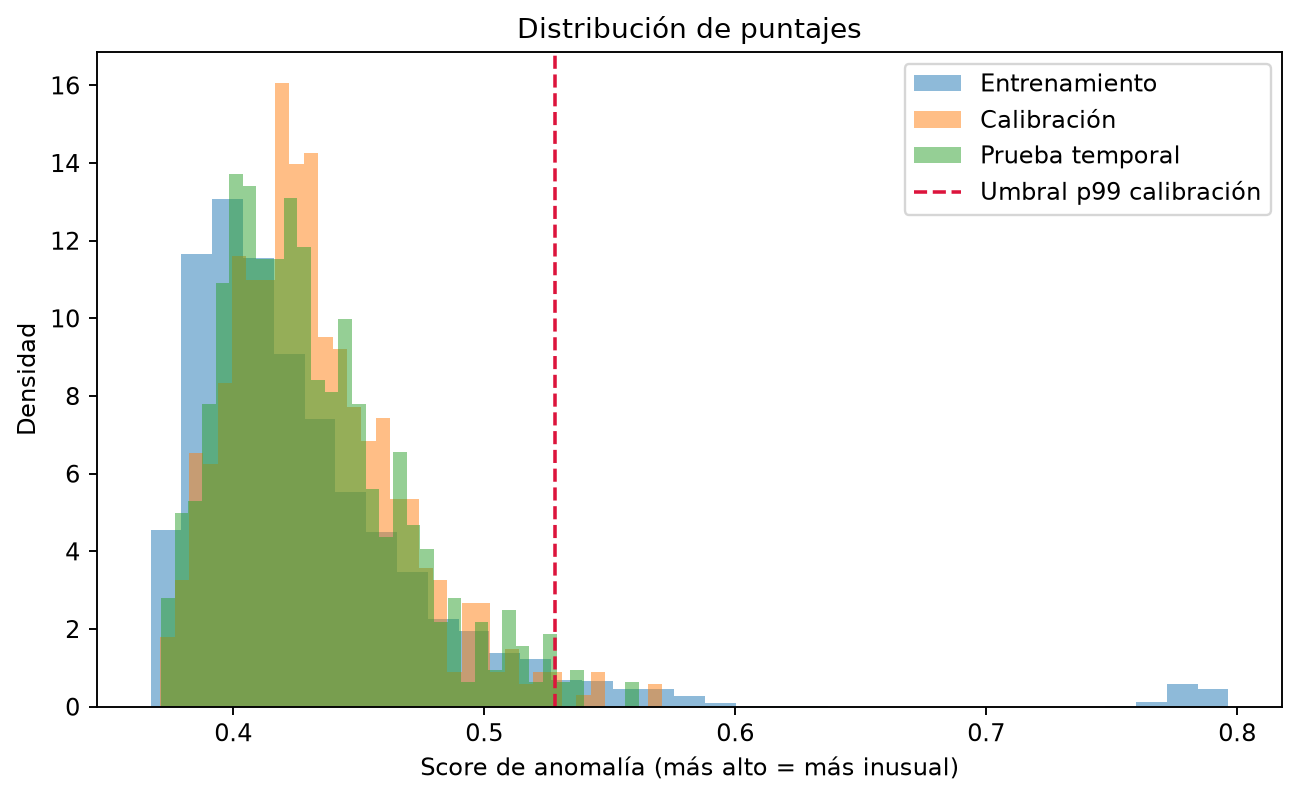
\includegraphics[width=\columnwidth]{imagenes/resultados/03_scores.png}
\caption{Distribución del puntaje de anomalía en entrenamiento, calibración y prueba. La línea
discontinua marca el umbral (percentil~99 de calibración, $s=0.528$).}
\label{fig:scores}
\end{figure}

En el bloque de prueba, el detector marcó como anómalas 7 de 590 lecturas (1.19\,\%), una tasa de
señalización sobre este bloque y no una medida de exactitud diagnóstica. El umbral p99 se estimó
con la calibración; por tanto, no garantiza una tasa de falsas alarmas del 1\,\% en futuras
sesiones. La Fig.~\ref{fig:temporal} muestra que esas
marcas aparecen aisladas: ninguna secuencia alcanzó tres anomalías seguidas, de modo que la regla
de persistencia no habría ordenado ninguna parada durante la operación normal. Hacia el final del
bloque el puntaje sube de forma sostenida hasta rozar el umbral; coincide con la caída de la tensión
del ACS712 por debajo de 1\,290~mV (Fig.~\ref{fig:senales}), un nivel ausente en el entrenamiento.
Es la primera evidencia de que el detector reacciona a desplazamientos de la corriente.

Para estimar el comportamiento de la regla de parada, se reprodujo la secuencia completa de 3\,927
lecturas tal como la recibiría la Lambda. En calibración (6 marcas) y en prueba (7 marcas) la
racha más larga fue de una sola lectura. La única secuencia que habría disparado la orden
\code{OFF} es el tramo inicial de 57 lecturas consecutivas, que corresponde a la reubicación del
MPU6050: un cambio real en la condición de montaje, correctamente señalado.

\begin{figure}[H]
\centering
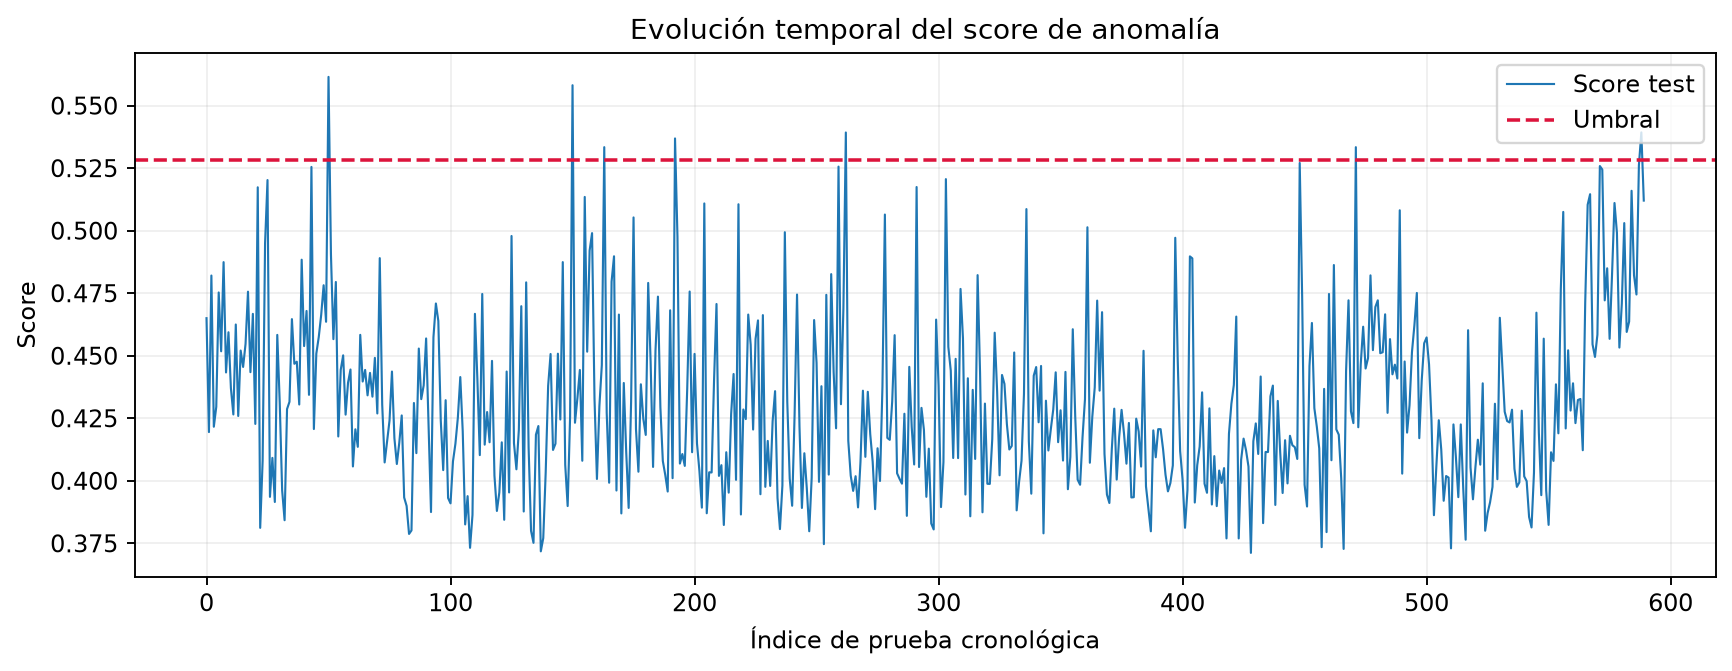
\includegraphics[width=\columnwidth]{imagenes/resultados/04_score_temporal.png}
\caption{Evolución del puntaje en el bloque de prueba cronológico (590 lecturas) frente al umbral.}
\label{fig:temporal}
\end{figure}

\subsection{Sensibilidad ante perturbaciones}

Para estimar la respuesta del detector ante desviaciones de magnitud creciente, se perturbaron las
lecturas de prueba con ruido cuya intensidad va de 0 a 100\,\% en pasos de 5 puntos. Para una
intensidad $p$, la perturbación se define como
\[
  \mathbf{x}_{p}=\mathbf{x}+\frac{p}{100}\,3\,\mathbf{s}\odot\boldsymbol{\epsilon},
\]
donde $\mathbf{s}$ contiene el rango intercuartílico de entrenamiento de cada variable (con la
desviación estándar como respaldo si ese rango es cero) y $\boldsymbol{\epsilon}$ es una dirección
gaussiana fija dentro de cada repetición. Así, 100\,\% representa tres veces esa escala estadística,
no una falla física de magnitud equivalente. El experimento se aplicó solo al conjunto de prueba y
se promediaron 12 repeticiones (Fig.~\ref{fig:ruido} y Tabla~\ref{tab:ruido}).

\begin{figure}[H]
\centering
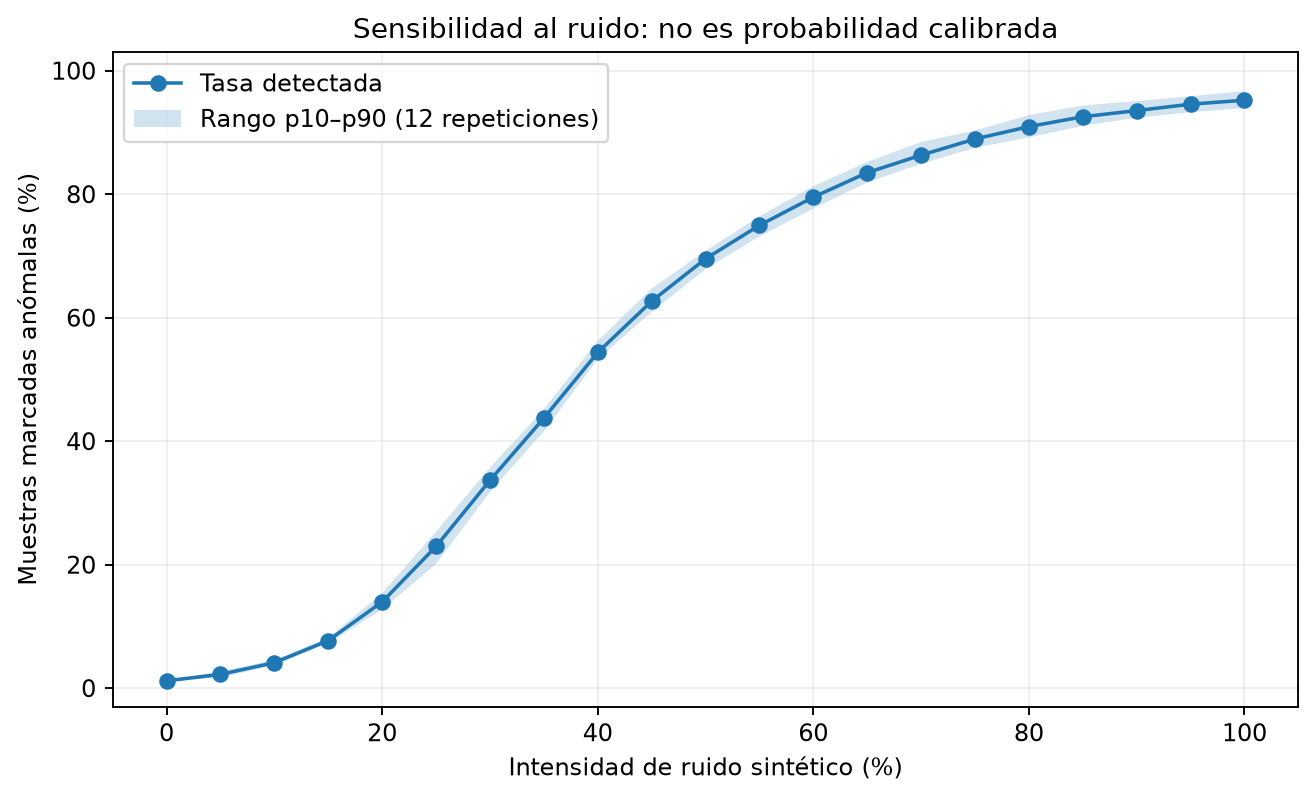
\includegraphics[width=\columnwidth]{imagenes/resultados/06_ruido_tasa_anomalias.png}
\caption{Porcentaje de lecturas marcadas como anómalas según la intensidad de la perturbación. La
banda indica el rango entre los percentiles 10 y 90 de 12 repeticiones.}
\label{fig:ruido}
\end{figure}

\begin{table}[htbp]
\centering
\caption{Respuesta del detector a perturbaciones sintéticas.}
\label{tab:ruido}
\footnotesize
\begin{tabular}{@{}rrrr@{}}
\toprule
\textbf{Ruido (\%)} & \textbf{Marcadas (\%)} & \textbf{p10--p90 (\%)} & \textbf{Mediana $s$} \\
\midrule
0 & 1.2 & 1.2--1.2 & 0.424 \\
10 & 4.1 & 3.7--4.6 & 0.441 \\
20 & 14.0 & 12.7--15.4 & 0.470 \\
30 & 33.7 & 31.7--35.7 & 0.505 \\
40 & 54.4 & 53.3--56.2 & 0.534 \\
50 & 69.5 & 67.9--70.8 & 0.558 \\
60 & 79.5 & 77.7--81.3 & 0.577 \\
80 & 90.9 & 89.2--92.8 & 0.604 \\
100 & 95.2 & 93.9--96.7 & 0.624 \\
\bottomrule
\end{tabular}
\end{table}

La tasa media de detección aumenta desde 1.19\,\% sin ruido hasta 54.36\,\% al 40\,\%,
90.95\,\% al 80\,\% y 95.23\,\% al 100\,\%. La mediana del puntaje sube de 0.424 a 0.624 y
supera el umbral de 0.5282 cerca del 38\,\% de intensidad. La banda p10--p90 es estrecha, aunque
este patrón describe únicamente las perturbaciones gaussianas del experimento; no es una relación
entre porcentaje de ruido y severidad de falla física, ni una probabilidad de avería.

\subsection{Verificación funcional de la cadena IoT}

La Tabla~\ref{tab:funcional} resume las pruebas de extremo a extremo.

\begin{table}[htbp]
\centering
\caption{Verificación funcional del prototipo.}
\label{tab:funcional}
\scriptsize
\begin{tabularx}{\columnwidth}{@{}>{\raggedright\arraybackslash}p{1.9cm}>{\raggedright\arraybackslash}X@{}}
\toprule
\textbf{Prueba} & \textbf{Resultado} \\
\midrule
Lectura de los tres sensores & 69~min de registro continuo a ${\sim}1$~Hz; 3\,927 lecturas
encendidas válidas; 5 reinicios del ESP32. \\
Control local del relé & Conmutación comprobada con los comandos \code{L}/\code{H} del monitor
serie; el estado se confirma con \code{S} (Anexo~\ref{anexo:evidencias-armado}). \\
Publicación MQTT/TLS & Conexión del \emph{thing} \code{esp32-26} por el puerto 8883; 50 lecturas
consecutivas recibidas en \code{esp32/pub} en 92~s (${\sim}1.8$~s por lectura). \\
Inferencia en Lambda & Una invocación por lectura desde la regla de IoT; ${\sim}84$~ms por
inferencia en caliente y 289~MB de memoria usados de 1\,024~MB (CloudWatch). \\
Registro en DynamoDB & Un ítem \code{PRED\#} por lectura y un ítem \code{STATE} por dispositivo;
el contador crece de uno en uno y \code{shutdown\_requested} se activa en la tercera anomalía
(Fig.~\ref{fig:dynamo}). \\
API y monitor web & \code{/api/latest} y \code{/api/history} respondieron \code{200} en
10--121~ms; \code{POST /api/command} sin clave fue rechazado con \code{401}. \\
Orden OFF $\rightarrow$ relé & Orden manual por la API: \code{202} en 0.48--0.85~s y apagado
confirmado en 3.6--7.2~s (media 5.3~s, tres ciclos); el encendido, en 3.7--4.1~s. \\
\bottomrule
\end{tabularx}
\end{table}

\subsection{Discusión y limitaciones}
\label{sec:discusion}

El resultado más importante es también la principal limitación. Con un ritmo de una lectura por
segundo, el MPU6050 entrega muestras instantáneas de la aceleración y no una descripción de la
vibración: un ventilador de este tipo gira a varios miles de revoluciones por minuto, es decir, a
decenas de hercios, y por el teorema de muestreo sus componentes vibratorias quedan fuera de
alcance. El P1 preveía calcular indicadores por ventana (RMS y factor de cresta) en el ESP32; esa
etapa no se implementó, y el detector actual reacciona sobre todo a cambios de orientación del
sensor y a desplazamientos de la corriente, como confirman las Figs.~\ref{fig:scores}
y~\ref{fig:temporal}.

Además, el conjunto de datos procede de una única sesión de una hora, sin fallas inducidas y
etiquetadas, por lo que no es posible estimar precisión ni sensibilidad frente a fallas reales; la
detección sintética del 83\,\% mide la sensibilidad a perturbaciones artificiales, no a desbalance o
fricción reales~\cite{lei2020}. Los registros consecutivos están correlacionados, de modo que la
partición cronológica reduce, pero no elimina, el optimismo de la evaluación. Finalmente, el
firmware actual no aplica límites físicos locales: si la conexión con AWS se pierde, el ventilador
solo puede detenerse por comando serie, en contra de lo recomendado en~\cite{compare2020}.

% =====================================================================
\section{Descripción del mercado}

El segmento objetivo son las pequeñas y medianas empresas industriales y de servicios que operan
máquinas rotativas de baja potencia ---ventiladores de extracción, bombas de agua, compresores y
motores de líneas de producción--- y que hoy dependen de inspecciones visuales o del mantenimiento
correctivo, porque las soluciones industriales de monitoreo de condición resultan costosas para su
escala. También se incluyen administradores de edificios con sistemas de ventilación y
laboratorios académicos que buscan una plataforma de enseñanza de mantenimiento predictivo.

El modelo de negocio propuesto combina la venta de un nodo de sensado de bajo costo con una
suscripción mensual por equipo monitoreado. La suscripción cubre la infraestructura en la nube,
cuyo costo escala con el número de mensajes gracias a los servicios sin servidor; el
reentrenamiento del modelo con la línea base de cada máquina del cliente; y el acceso a alertas e
historial. Como servicio adicional, se ofrecería la instalación y la calibración en planta,
cobrada por proyecto.

% =====================================================================
\section{Conclusiones y recomendaciones}

\subsection{Conclusiones}
\begin{enumerate}
  \item Se implementó un prototipo IoT que integra tres sensores, un ESP32, comunicación MQTT
        sobre TLS, inferencia sin servidores en AWS y un relé de parada, con lo que se cubren
        todos los requisitos mínimos del curso.
  \item Se construyó un conjunto de datos real de 4\,261 lecturas (3\,927 con el ventilador
        reportado como ENCENDIDO) y se entrenó un detector Isolation Forest con partición
        cronológica. El 1.19\,\% de señalización en las 590 lecturas de prueba describe ese bloque,
        no una exactitud sobre fallas reales; ENCENDIDO tampoco certifica salud.
  \item Ante perturbaciones sintéticas, la tasa media de señalización creció de 1.19\,\% sin
        perturbación a 95.23\,\% con la intensidad máxima definida. Esto demuestra respuesta a
        cambios artificiales en las variables, no sensibilidad comprobada ante fallas físicas.
  \item Sustituir RCF por Isolation Forest y la laptop por AWS Lambda permitió desplegar el modelo
        sin un punto de inferencia permanente y con autenticación por certificado, a cambio de
        depender de la conectividad para la decisión remota.
  \item El muestreo a 1~Hz y la falta de fallas etiquetadas impiden afirmar que el sistema detecta
        desbalance o fricción reales; lo demostrado es la cadena completa de adquisición,
        inferencia y actuación, y la respuesta del detector a desviaciones de las variables.
\end{enumerate}

\subsection{Recomendaciones}
\begin{enumerate}
  \item Separar la lectura del DS18B20 (asíncrona, cada pocos segundos) de la del MPU6050 y
        muestrear este último a cientos de hercios, calculando en el ESP32 RMS, pico y factor de
        cresta por ventana, como proponía el P1.
  \item Registrar sesiones con fallas inducidas y etiquetadas (masa adherida a un aspa, rozamiento
        del eje, obstrucción del flujo) para medir sensibilidad y precisión reales.
  \item Añadir en el firmware límites locales de corriente y temperatura con histéresis, de modo
        que la protección no dependa de la nube.
  \item Incorporar la lectura del tacómetro del ventilador como variable de contexto y entrenar con
        varias sesiones para capturar la variabilidad entre arranques.
  \item Integrar la API de consulta en el gemelo digital 3D y añadir al monitor web la variable
        que más contribuye a cada anomalía.
\end{enumerate}

% =====================================================================
\balance
\renewcommand{\refname}{Referencias bibliográficas}
\begin{thebibliography}{99}
\footnotesize
\setlength{\itemsep}{1pt}

\bibitem{tiboni2022}
M. Tiboni, C. Remino, R. Bussola, and C. Amici, ``A review on vibration-based condition
monitoring of rotating machinery,'' \emph{Appl. Sci.}, vol.~12, no.~3, Art. no.~972, Jan. 2022,
doi: 10.3390/app12030972.

\bibitem{lei2018}
Y. Lei, N. Li, L. Guo, N. Li, T. Yan, and J. Lin, ``Machinery health prognostics: A systematic
review from data acquisition to RUL prediction,'' \emph{Mech. Syst. Signal Process.}, vol.~104,
pp.~799--834, May 2018, doi: 10.1016/j.ymssp.2017.11.016.

\bibitem{compare2020}
M. Compare, P. Baraldi, and E. Zio, ``Challenges to IoT-enabled predictive maintenance for
Industry 4.0,'' \emph{IEEE Internet Things J.}, vol.~7, no.~5, pp.~4585--4597, May 2020,
doi: 10.1109/JIOT.2019.2957029.

\bibitem{zonta2020}
T. Zonta, C. A. da Costa, R. da Rosa Righi, M. J. de Lima, E. S. da Trindade, and G. P. Li,
``Predictive maintenance in the Industry 4.0: A systematic literature review,'' \emph{Comput. Ind.
Eng.}, vol.~150, Art. no.~106889, Dec. 2020, doi: 10.1016/j.cie.2020.106889.

\bibitem{carvalho2019}
T. P. Carvalho, F. A. A. M. N. Soares, R. Vita, R. da P. Francisco, J. P. Basto, and
S. G. S. Alcalá, ``A systematic literature review of machine learning methods applied to
predictive maintenance,'' \emph{Comput. Ind. Eng.}, vol.~137, Art. no.~106024, Nov. 2019,
doi: 10.1016/j.cie.2019.106024.

\bibitem{cinar2020}
Z. M. \c{C}{\i}nar, A. Abdussalam Nuhu, Q. Zeeshan, O. Korhan, M. Asmael, and B. Safaei, ``Machine
learning in predictive maintenance towards sustainable smart manufacturing in Industry 4.0,''
\emph{Sustainability}, vol.~12, no.~19, Art. no.~8211, Oct. 2020, doi: 10.3390/su12198211.

\bibitem{li2017}
X. Li, F. Duan, D. Mba, and I. Bennett, ``Multidimensional prognostics for rotating machinery: A
review,'' \emph{Adv. Mech. Eng.}, vol.~9, no.~2, pp.~1--20, Feb. 2017,
doi: 10.1177/1687814016685004.

\bibitem{niu2023}
G. Niu, X. Dong, and Y. Chen, ``Motor fault diagnostics based on current signatures: A review,''
\emph{IEEE Trans. Instrum. Meas.}, vol.~72, Art. no.~3520919, 2023,
doi: 10.1109/TIM.2023.3285999.

\bibitem{zhang2019}
W. Zhang, D. Yang, and H. Wang, ``Data-driven methods for predictive maintenance of industrial
equipment: A survey,'' \emph{IEEE Syst. J.}, vol.~13, no.~3, pp.~2213--2227, Sep. 2019,
doi: 10.1109/JSYST.2019.2905565.

\bibitem{mpu6050}
InvenSense Inc., ``MPU-6000 and MPU-6050 product specification,'' Rev.~3.4, Aug. 2013. [Online].
Available: \url{https://invensense.tdk.com/wp-content/uploads/2015/02/MPU-6000-Datasheet1.pdf}

\bibitem{acs712}
Allegro MicroSystems, ``ACS712: Fully integrated, Hall-effect-based linear current sensor IC with
2.1~kVRMS isolation and a low-resistance current conductor,'' datasheet. [Online]. Available:
\url{https://www.allegromicro.com/-/media/files/datasheets/acs712-datasheet.pdf}

\bibitem{benbouzid2000}
M. E. H. Benbouzid, ``A review of induction motors signature analysis as a medium for faults
detection,'' \emph{IEEE Trans. Ind. Electron.}, vol.~47, no.~5, pp.~984--993, Oct. 2000,
doi: 10.1109/41.873206.

\bibitem{ds18b20}
Analog Devices, ``DS18B20 programmable resolution 1-Wire digital thermometer,'' Rev.~6, 2019.
[Online]. Available:
\url{https://www.analog.com/media/en/technical-documentation/data-sheets/DS18B20.pdf}

\bibitem{liu2008}
F. T. Liu, K. M. Ting, and Z.-H. Zhou, ``Isolation forest,'' in \emph{Proc. 8th IEEE Int. Conf.
Data Mining (ICDM)}, Pisa, Italy, 2008, pp.~413--422, doi: 10.1109/ICDM.2008.17.

\bibitem{liu2012}
F. T. Liu, K. M. Ting, and Z.-H. Zhou, ``Isolation-based anomaly detection,'' \emph{ACM Trans.
Knowl. Discov. Data}, vol.~6, no.~1, Art. no.~3, Mar. 2012, doi: 10.1145/2133360.2133363.

\bibitem{guha2016}
S. Guha, N. Mishra, G. Roy, and O. Schrijvers, ``Robust random cut forest based anomaly detection
on streams,'' in \emph{Proc. 33rd Int. Conf. Mach. Learn. (ICML)}, New York, NY, USA, 2016,
pp.~2712--2721.

\bibitem{mqtt311}
A. Banks and R. Gupta, Eds., ``MQTT version 3.1.1,'' OASIS Standard, Oct. 2014. [Online].
Available: \url{https://docs.oasis-open.org/mqtt/mqtt/v3.1.1/mqtt-v3.1.1.html}

\bibitem{mishra2020}
B. Mishra and A. Kertesz, ``The use of MQTT in M2M and IoT systems: A survey,'' \emph{IEEE
Access}, vol.~8, pp.~201071--201086, 2020, doi: 10.1109/ACCESS.2020.3035849.

\bibitem{awsiot}
Amazon Web Services, ``What is AWS IoT?,'' \emph{AWS IoT Core Developer Guide}. [Online].
Available: \url{https://docs.aws.amazon.com/iot/latest/developerguide/what-is-aws-iot.html}
(accessed Nov.~13, 2026).

\bibitem{awsrules}
Amazon Web Services, ``Rules for AWS IoT,'' \emph{AWS IoT Core Developer Guide}. [Online].
Available: \url{https://docs.aws.amazon.com/iot/latest/developerguide/iot-rules.html}
(accessed Nov.~13, 2026).

\bibitem{awslambda}
Amazon Web Services, ``Create a Lambda function using a container image,'' \emph{AWS Lambda
Developer Guide}. [Online]. Available:
\url{https://docs.aws.amazon.com/lambda/latest/dg/images-create.html} (accessed Nov.~13, 2026).

\bibitem{lei2020}
Y. Lei, B. Yang, X. Jiang, F. Jia, N. Li, and A. K. Nandi, ``Applications of machine learning to
machine fault diagnosis: A review and roadmap,'' \emph{Mech. Syst. Signal Process.}, vol.~138,
Art. no.~106587, Apr. 2020, doi: 10.1016/j.ymssp.2019.106587.

\bibitem{serradilla2022}
O. Serradilla, E. Zugasti, J. Rodriguez, and U. Zurutuza, ``Deep learning models for predictive
maintenance: A survey, comparison, challenges and prospects,'' \emph{Appl. Intell.}, vol.~52,
no.~10, pp.~10934--10964, 2022, doi: 10.1007/s10489-021-03004-y.

\bibitem{pang2021}
G. Pang, C. Shen, L. Cao, and A. van den Hengel, ``Deep learning for anomaly detection: A
review,'' \emph{ACM Comput. Surv.}, vol.~54, no.~2, Art. no.~38, Mar. 2021,
doi: 10.1145/3439950.

\bibitem{hariri2021}
S. Hariri, M. Carrasco Kind, and R. J. Brunner, ``Extended isolation forest,'' \emph{IEEE Trans.
Knowl. Data Eng.}, vol.~33, no.~4, pp.~1479--1489, Apr. 2021, doi: 10.1109/TKDE.2019.2947676.

\bibitem{esp32}
Espressif Systems, ``ESP32 series datasheet,'' Ver.~5.3, 2026. [Online]. Available:
\url{https://www.espressif.com/sites/default/files/documentation/esp32_datasheet_en.pdf}

\bibitem{awsrcf}
Amazon Web Services, ``How RCF works,'' \emph{Amazon SageMaker AI Developer Guide}. [Online].
Available: \url{https://docs.aws.amazon.com/sagemaker/latest/dg/rcf_how-it-works.html}
(accessed Nov.~13, 2026).

\bibitem{sklearn}
F. Pedregosa \emph{et al.}, ``Scikit-learn: Machine learning in Python,'' \emph{J. Mach. Learn.
Res.}, vol.~12, pp.~2825--2830, 2011.

\bibitem{wokwi}
Wokwi, ``Wokwi documentation: ESP32 simulation.'' [Online]. Available:
\url{https://docs.wokwi.com} (accessed Nov.~13, 2026).

\end{thebibliography}

\section*{Anexos}
\appendix
\titleformat{\section}{\normalsize\bfseries\color{GrisTexto}}{\thesection.}{0.45em}{}
\section{Evidencias del armado}
\label{anexo:evidencias-armado}

La \href{https://drive.google.com/drive/folders/1GaprwriotHJuRfBhnqh_3qpv-3r5A804?usp=sharing}{carpeta de Drive}
reúne los dos videos del prototipo y el archivo \code{sketch\_nov6a.ino}
usado en la prueba por puerto serie.

\end{document}